% Options for packages loaded elsewhere
\PassOptionsToPackage{unicode}{hyperref}
\PassOptionsToPackage{hyphens}{url}
%
\documentclass[
]{article}
\usepackage{amsmath,amssymb}
\usepackage{iftex}
\ifPDFTeX
  \usepackage[T1]{fontenc}
  \usepackage[utf8]{inputenc}
  \usepackage{textcomp} % provide euro and other symbols
\else % if luatex or xetex
  \usepackage{unicode-math} % this also loads fontspec
  \defaultfontfeatures{Scale=MatchLowercase}
  \defaultfontfeatures[\rmfamily]{Ligatures=TeX,Scale=1}
\fi
\usepackage{lmodern}
\ifPDFTeX\else
  % xetex/luatex font selection
\fi
% Use upquote if available, for straight quotes in verbatim environments
\IfFileExists{upquote.sty}{\usepackage{upquote}}{}
\IfFileExists{microtype.sty}{% use microtype if available
  \usepackage[]{microtype}
  \UseMicrotypeSet[protrusion]{basicmath} % disable protrusion for tt fonts
}{}
\makeatletter
\@ifundefined{KOMAClassName}{% if non-KOMA class
  \IfFileExists{parskip.sty}{%
    \usepackage{parskip}
  }{% else
    \setlength{\parindent}{0pt}
    \setlength{\parskip}{6pt plus 2pt minus 1pt}}
}{% if KOMA class
  \KOMAoptions{parskip=half}}
\makeatother
\usepackage{xcolor}
\usepackage[margin=1in]{geometry}
\usepackage{color}
\usepackage{fancyvrb}
\newcommand{\VerbBar}{|}
\newcommand{\VERB}{\Verb[commandchars=\\\{\}]}
\DefineVerbatimEnvironment{Highlighting}{Verbatim}{commandchars=\\\{\}}
% Add ',fontsize=\small' for more characters per line
\usepackage{framed}
\definecolor{shadecolor}{RGB}{248,248,248}
\newenvironment{Shaded}{\begin{snugshade}}{\end{snugshade}}
\newcommand{\AlertTok}[1]{\textcolor[rgb]{0.94,0.16,0.16}{#1}}
\newcommand{\AnnotationTok}[1]{\textcolor[rgb]{0.56,0.35,0.01}{\textbf{\textit{#1}}}}
\newcommand{\AttributeTok}[1]{\textcolor[rgb]{0.13,0.29,0.53}{#1}}
\newcommand{\BaseNTok}[1]{\textcolor[rgb]{0.00,0.00,0.81}{#1}}
\newcommand{\BuiltInTok}[1]{#1}
\newcommand{\CharTok}[1]{\textcolor[rgb]{0.31,0.60,0.02}{#1}}
\newcommand{\CommentTok}[1]{\textcolor[rgb]{0.56,0.35,0.01}{\textit{#1}}}
\newcommand{\CommentVarTok}[1]{\textcolor[rgb]{0.56,0.35,0.01}{\textbf{\textit{#1}}}}
\newcommand{\ConstantTok}[1]{\textcolor[rgb]{0.56,0.35,0.01}{#1}}
\newcommand{\ControlFlowTok}[1]{\textcolor[rgb]{0.13,0.29,0.53}{\textbf{#1}}}
\newcommand{\DataTypeTok}[1]{\textcolor[rgb]{0.13,0.29,0.53}{#1}}
\newcommand{\DecValTok}[1]{\textcolor[rgb]{0.00,0.00,0.81}{#1}}
\newcommand{\DocumentationTok}[1]{\textcolor[rgb]{0.56,0.35,0.01}{\textbf{\textit{#1}}}}
\newcommand{\ErrorTok}[1]{\textcolor[rgb]{0.64,0.00,0.00}{\textbf{#1}}}
\newcommand{\ExtensionTok}[1]{#1}
\newcommand{\FloatTok}[1]{\textcolor[rgb]{0.00,0.00,0.81}{#1}}
\newcommand{\FunctionTok}[1]{\textcolor[rgb]{0.13,0.29,0.53}{\textbf{#1}}}
\newcommand{\ImportTok}[1]{#1}
\newcommand{\InformationTok}[1]{\textcolor[rgb]{0.56,0.35,0.01}{\textbf{\textit{#1}}}}
\newcommand{\KeywordTok}[1]{\textcolor[rgb]{0.13,0.29,0.53}{\textbf{#1}}}
\newcommand{\NormalTok}[1]{#1}
\newcommand{\OperatorTok}[1]{\textcolor[rgb]{0.81,0.36,0.00}{\textbf{#1}}}
\newcommand{\OtherTok}[1]{\textcolor[rgb]{0.56,0.35,0.01}{#1}}
\newcommand{\PreprocessorTok}[1]{\textcolor[rgb]{0.56,0.35,0.01}{\textit{#1}}}
\newcommand{\RegionMarkerTok}[1]{#1}
\newcommand{\SpecialCharTok}[1]{\textcolor[rgb]{0.81,0.36,0.00}{\textbf{#1}}}
\newcommand{\SpecialStringTok}[1]{\textcolor[rgb]{0.31,0.60,0.02}{#1}}
\newcommand{\StringTok}[1]{\textcolor[rgb]{0.31,0.60,0.02}{#1}}
\newcommand{\VariableTok}[1]{\textcolor[rgb]{0.00,0.00,0.00}{#1}}
\newcommand{\VerbatimStringTok}[1]{\textcolor[rgb]{0.31,0.60,0.02}{#1}}
\newcommand{\WarningTok}[1]{\textcolor[rgb]{0.56,0.35,0.01}{\textbf{\textit{#1}}}}
\usepackage{graphicx}
\makeatletter
\def\maxwidth{\ifdim\Gin@nat@width>\linewidth\linewidth\else\Gin@nat@width\fi}
\def\maxheight{\ifdim\Gin@nat@height>\textheight\textheight\else\Gin@nat@height\fi}
\makeatother
% Scale images if necessary, so that they will not overflow the page
% margins by default, and it is still possible to overwrite the defaults
% using explicit options in \includegraphics[width, height, ...]{}
\setkeys{Gin}{width=\maxwidth,height=\maxheight,keepaspectratio}
% Set default figure placement to htbp
\makeatletter
\def\fps@figure{htbp}
\makeatother
\setlength{\emergencystretch}{3em} % prevent overfull lines
\providecommand{\tightlist}{%
  \setlength{\itemsep}{0pt}\setlength{\parskip}{0pt}}
\setcounter{secnumdepth}{-\maxdimen} % remove section numbering
\ifLuaTeX
  \usepackage{selnolig}  % disable illegal ligatures
\fi
\usepackage{bookmark}
\IfFileExists{xurl.sty}{\usepackage{xurl}}{} % add URL line breaks if available
\urlstyle{same}
\hypersetup{
  hidelinks,
  pdfcreator={LaTeX via pandoc}}

\author{}
\date{\vspace{-2.5em}}

\begin{document}

\section{Replace with Main Title}\label{replace-with-main-title}

\subsubsection{mihap}\label{mihap}

\subsubsection{2024-10-10}\label{section}

\begin{verbatim}
## Loading required package: splines
\end{verbatim}

\begin{verbatim}
## Loading required package: RcmdrMisc
\end{verbatim}

\begin{verbatim}
## Loading required package: car
\end{verbatim}

\begin{verbatim}
## Loading required package: carData
\end{verbatim}

\begin{verbatim}
## Loading required package: sandwich
\end{verbatim}

\begin{verbatim}
## Loading required package: effects
\end{verbatim}

\begin{verbatim}
## lattice theme set by effectsTheme()
## See ?effectsTheme for details.
\end{verbatim}

\begin{verbatim}
## The Commander GUI is launched only in interactive sessions
\end{verbatim}

\begin{verbatim}
## 
## Attaching package: 'Rcmdr'
\end{verbatim}

\begin{verbatim}
## The following object is masked from 'package:base':
## 
##     errorCondition
\end{verbatim}

\begin{Shaded}
\begin{Highlighting}[]
\SpecialCharTok{\textgreater{}}\NormalTok{ my.data }\OtherTok{\textless{}{-}} 
\SpecialCharTok{+}   \FunctionTok{read.table}\NormalTok{(}\StringTok{"C:/Users/mihap/Code/Faks/famnit24{-}statistika/practice/data.txt"}\NormalTok{,}
\SpecialCharTok{+}    \AttributeTok{header=}\ConstantTok{TRUE}\NormalTok{, }\AttributeTok{stringsAsFactors=}\ConstantTok{TRUE}\NormalTok{, }\AttributeTok{sep=}\StringTok{"}\SpecialCharTok{\textbackslash{}t}\StringTok{"}\NormalTok{, }\AttributeTok{na.strings=}\StringTok{"NA"}\NormalTok{, }\AttributeTok{dec=}\StringTok{"."}\NormalTok{, }
\SpecialCharTok{+}   \AttributeTok{strip.white=}\ConstantTok{TRUE}\NormalTok{)}
\end{Highlighting}
\end{Shaded}

\subsubsection{Summarize Data Set:
my.data}\label{summarize-data-set-my.data}

\begin{Shaded}
\begin{Highlighting}[]
\SpecialCharTok{\textgreater{}} \FunctionTok{summary}\NormalTok{(my.data)}
\end{Highlighting}
\end{Shaded}

\begin{verbatim}
               Timestamp        Age            Sex          Height     
 10.10.2010 10:38:39:  1   Min.   :18.00   female:348   Min.   :152.0  
 10.10.2010 14:13:31:  1   1st Qu.:20.00   male  :176   1st Qu.:167.0  
 10.10.2010 17:30:55:  1   Median :20.00                Median :171.0  
 10.10.2010 17:54:13:  1   Mean   :20.06                Mean   :173.2  
 10.10.2010 21:32:16:  1   3rd Qu.:20.00                3rd Qu.:179.0  
 10.11.2010 18:58:17:  1   Max.   :27.00                Max.   :202.0  
 (Other)            :518                                               
     Weight         Shoe.size     Eye.Color   Smoking  
 Min.   : 31.00   Min.   :35.00   black:  6   no :483  
 1st Qu.: 57.00   1st Qu.:38.00   blue :148   yes: 41  
 Median : 64.00   Median :40.00   brown:223            
 Mean   : 65.64   Mean   :40.42   green:117            
 3rd Qu.: 74.00   3rd Qu.:42.00   other: 30            
 Max.   :103.00   Max.   :49.00                        
 NA's   :1                                             
 Smoking.How.many.per.day Videogames TV..hours.per.week.
 Min.   : 0.0000          no :370    Min.   : 0.000     
 1st Qu.: 0.0000          yes:154    1st Qu.: 2.000     
 Median : 0.0000                     Median : 4.000     
 Mean   : 0.5919                     Mean   : 5.256     
 3rd Qu.: 0.0000                     3rd Qu.: 7.000     
 Max.   :25.0000                     Max.   :45.000     
                                                        
 Internet..hours.per.week. Books..how.many.per.year. Sport..hours.per.week.
 Min.   : 1.00             Min.   :  0.00            Min.   : 0.000        
 1st Qu.: 7.00             1st Qu.:  5.00            1st Qu.: 3.000        
 Median :12.00             Median :  8.00            Median : 4.000        
 Mean   :15.35             Mean   : 11.59            Mean   : 5.417        
 3rd Qu.:20.00             3rd Qu.: 15.00            3rd Qu.: 7.000        
 Max.   :80.00             Max.   :150.00            Max.   :30.000        
                           NA's   :2                                       
       Pet                 Faculty    Friends.on.Facebook
 no      :152   Dental Medicine: 73   Min.   :   0       
 Dog     :105   Medicine       :352   1st Qu.: 152       
 Cat     : 71   Veterinary     : 99   Median : 300       
 Cat, Dog: 41                         Mean   : 326       
 Other   : 23                         3rd Qu.: 431       
 Rodent  : 20                         Max.   :5000       
 (Other) :112                         NA's   :277        
 Sleep..hours.per.night. PetBird   PetCat    PetDog    PetFish   Petno    
 Min.   : 4.000          No :495   No :350   No :311   No :473   No :371  
 1st Qu.: 7.000          Yes: 29   Yes:174   Yes:213   Yes: 51   Yes:153  
 Median : 7.000                                                           
 Mean   : 7.304                                                           
 3rd Qu.: 8.000                                                           
 Max.   :12.000                                                           
 NA's   :277                                                              
 PetOther  PetRodent
 No :449   No :478  
 Yes: 75   Yes: 46  
                    
                    
                    
                    
                    
\end{verbatim}

\begin{Shaded}
\begin{Highlighting}[]
\SpecialCharTok{\textgreater{}} \FunctionTok{library}\NormalTok{(abind, }\AttributeTok{pos=}\DecValTok{17}\NormalTok{)}
\end{Highlighting}
\end{Shaded}

\begin{Shaded}
\begin{Highlighting}[]
\SpecialCharTok{\textgreater{}} \FunctionTok{library}\NormalTok{(e1071, }\AttributeTok{pos=}\DecValTok{18}\NormalTok{)}
\end{Highlighting}
\end{Shaded}

\subsubsection{Numerical Summaries:
my.data}\label{numerical-summaries-my.data}

\begin{Shaded}
\begin{Highlighting}[]
\SpecialCharTok{\textgreater{}}\NormalTok{ Dataset }\OtherTok{\textless{}{-}} 
\SpecialCharTok{+}   \FunctionTok{read.table}\NormalTok{(}\StringTok{"C:/Users/mihap/Code/Faks/famnit24{-}statistika/practice/data.txt"}\NormalTok{,}
\SpecialCharTok{+}    \AttributeTok{header=}\ConstantTok{TRUE}\NormalTok{, }\AttributeTok{stringsAsFactors=}\ConstantTok{TRUE}\NormalTok{, }\AttributeTok{sep=}\StringTok{"}\SpecialCharTok{\textbackslash{}t}\StringTok{"}\NormalTok{, }\AttributeTok{na.strings=}\StringTok{"NA"}\NormalTok{, }\AttributeTok{dec=}\StringTok{"."}\NormalTok{, }
\SpecialCharTok{+}   \AttributeTok{strip.white=}\ConstantTok{TRUE}\NormalTok{)}
\end{Highlighting}
\end{Shaded}

\subsubsection{Summarize Data Set:
Dataset}\label{summarize-data-set-dataset}

\begin{Shaded}
\begin{Highlighting}[]
\SpecialCharTok{\textgreater{}} \FunctionTok{summary}\NormalTok{(Dataset)}
\end{Highlighting}
\end{Shaded}

\begin{verbatim}
               Timestamp        Age            Sex          Height     
 10.10.2010 10:38:39:  1   Min.   :18.00   female:348   Min.   :152.0  
 10.10.2010 14:13:31:  1   1st Qu.:20.00   male  :176   1st Qu.:167.0  
 10.10.2010 17:30:55:  1   Median :20.00                Median :171.0  
 10.10.2010 17:54:13:  1   Mean   :20.06                Mean   :173.2  
 10.10.2010 21:32:16:  1   3rd Qu.:20.00                3rd Qu.:179.0  
 10.11.2010 18:58:17:  1   Max.   :27.00                Max.   :202.0  
 (Other)            :518                                               
     Weight         Shoe.size     Eye.Color   Smoking  
 Min.   : 31.00   Min.   :35.00   black:  6   no :483  
 1st Qu.: 57.00   1st Qu.:38.00   blue :148   yes: 41  
 Median : 64.00   Median :40.00   brown:223            
 Mean   : 65.64   Mean   :40.42   green:117            
 3rd Qu.: 74.00   3rd Qu.:42.00   other: 30            
 Max.   :103.00   Max.   :49.00                        
 NA's   :1                                             
 Smoking.How.many.per.day Videogames TV..hours.per.week.
 Min.   : 0.0000          no :370    Min.   : 0.000     
 1st Qu.: 0.0000          yes:154    1st Qu.: 2.000     
 Median : 0.0000                     Median : 4.000     
 Mean   : 0.5919                     Mean   : 5.256     
 3rd Qu.: 0.0000                     3rd Qu.: 7.000     
 Max.   :25.0000                     Max.   :45.000     
                                                        
 Internet..hours.per.week. Books..how.many.per.year. Sport..hours.per.week.
 Min.   : 1.00             Min.   :  0.00            Min.   : 0.000        
 1st Qu.: 7.00             1st Qu.:  5.00            1st Qu.: 3.000        
 Median :12.00             Median :  8.00            Median : 4.000        
 Mean   :15.35             Mean   : 11.59            Mean   : 5.417        
 3rd Qu.:20.00             3rd Qu.: 15.00            3rd Qu.: 7.000        
 Max.   :80.00             Max.   :150.00            Max.   :30.000        
                           NA's   :2                                       
       Pet                 Faculty    Friends.on.Facebook
 no      :152   Dental Medicine: 73   Min.   :   0       
 Dog     :105   Medicine       :352   1st Qu.: 152       
 Cat     : 71   Veterinary     : 99   Median : 300       
 Cat, Dog: 41                         Mean   : 326       
 Other   : 23                         3rd Qu.: 431       
 Rodent  : 20                         Max.   :5000       
 (Other) :112                         NA's   :277        
 Sleep..hours.per.night. PetBird   PetCat    PetDog    PetFish   Petno    
 Min.   : 4.000          No :495   No :350   No :311   No :473   No :371  
 1st Qu.: 7.000          Yes: 29   Yes:174   Yes:213   Yes: 51   Yes:153  
 Median : 7.000                                                           
 Mean   : 7.304                                                           
 3rd Qu.: 8.000                                                           
 Max.   :12.000                                                           
 NA's   :277                                                              
 PetOther  PetRodent
 No :449   No :478  
 Yes: 75   Yes: 46  
                    
                    
                    
                    
                    
\end{verbatim}

\subsubsection{Histogram:
Sport..hours.per.week.}\label{histogram-sport..hours.per.week.}

\begin{Shaded}
\begin{Highlighting}[]
\SpecialCharTok{\textgreater{}} \FunctionTok{with}\NormalTok{(Dataset, }\FunctionTok{Hist}\NormalTok{(Sport..hours.per.week., }\AttributeTok{scale=}\StringTok{"frequency"}\NormalTok{, }
\SpecialCharTok{+}   \AttributeTok{breaks=}\StringTok{"Sturges"}\NormalTok{, }\AttributeTok{col=}\StringTok{"darkgray"}\NormalTok{))}
\end{Highlighting}
\end{Shaded}

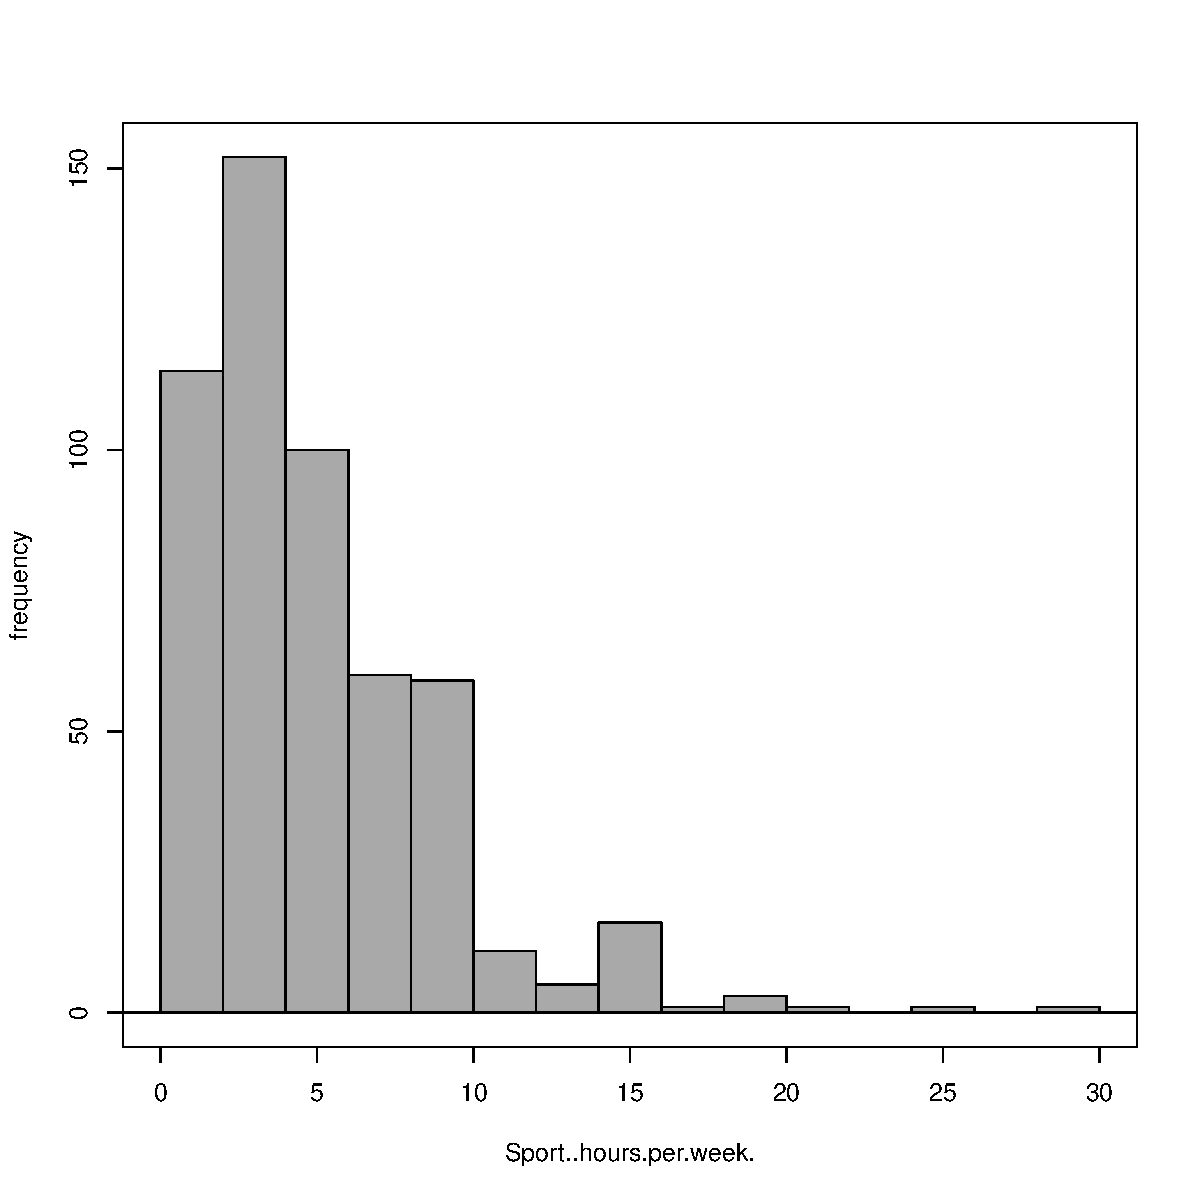
\includegraphics[width=750px]{RcmdrMarkdown_files/figure-latex/unnamed-chunk-8-1}

\subsubsection{Histogram:
Sport..hours.per.week.}\label{histogram-sport..hours.per.week.-1}

\begin{Shaded}
\begin{Highlighting}[]
\SpecialCharTok{\textgreater{}} \FunctionTok{with}\NormalTok{(Dataset, }\FunctionTok{Hist}\NormalTok{(Sport..hours.per.week., }\AttributeTok{scale=}\StringTok{"frequency"}\NormalTok{, }
\SpecialCharTok{+}   \AttributeTok{breaks=}\StringTok{"Sturges"}\NormalTok{, }\AttributeTok{col=}\StringTok{"darkgray"}\NormalTok{, }\AttributeTok{xlab=}\StringTok{"Št. ur športa na teden"}\NormalTok{, }
\SpecialCharTok{+}   \AttributeTok{ylab=}\StringTok{"Frekvenca"}\NormalTok{))}
\end{Highlighting}
\end{Shaded}

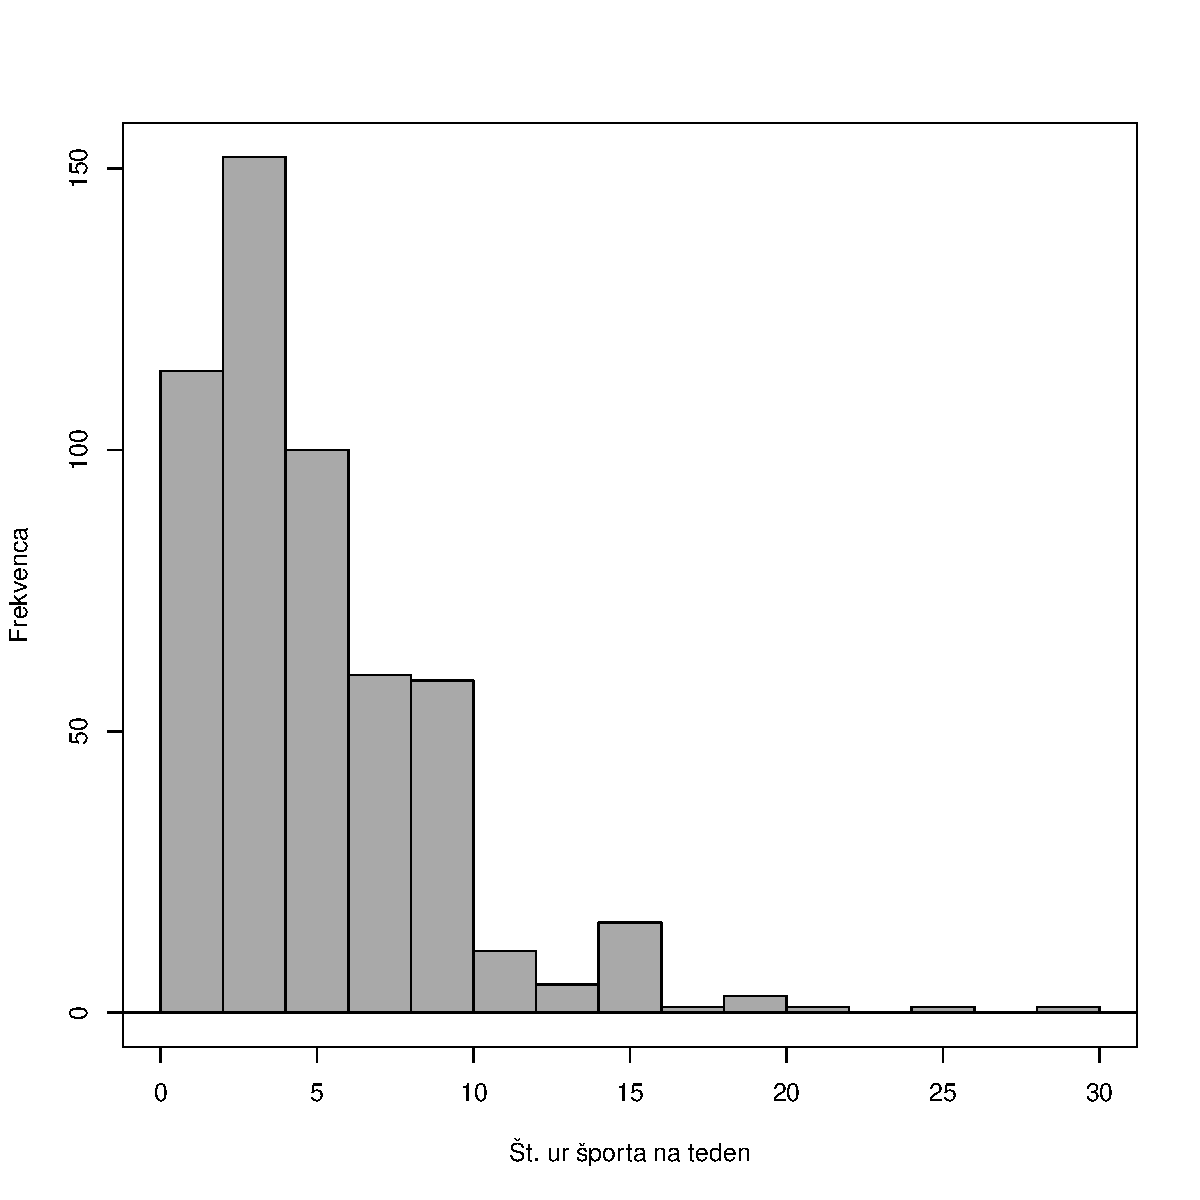
\includegraphics[width=750px]{RcmdrMarkdown_files/figure-latex/unnamed-chunk-9-1}

\subsubsection{Histogram:
Sport..hours.per.week.}\label{histogram-sport..hours.per.week.-2}

\begin{Shaded}
\begin{Highlighting}[]
\SpecialCharTok{\textgreater{}} \FunctionTok{with}\NormalTok{(Dataset, }\FunctionTok{Hist}\NormalTok{(Sport..hours.per.week., }\AttributeTok{scale=}\StringTok{"frequency"}\NormalTok{, }
\SpecialCharTok{+}   \AttributeTok{breaks=}\StringTok{"Sturges"}\NormalTok{, }\AttributeTok{col=}\StringTok{"darkgray"}\NormalTok{, }\AttributeTok{xlab=}\StringTok{"Št. ur športa na teden"}\NormalTok{, }
\SpecialCharTok{+}   \AttributeTok{ylab=}\StringTok{"Frekvenca"}\NormalTok{))}
\end{Highlighting}
\end{Shaded}

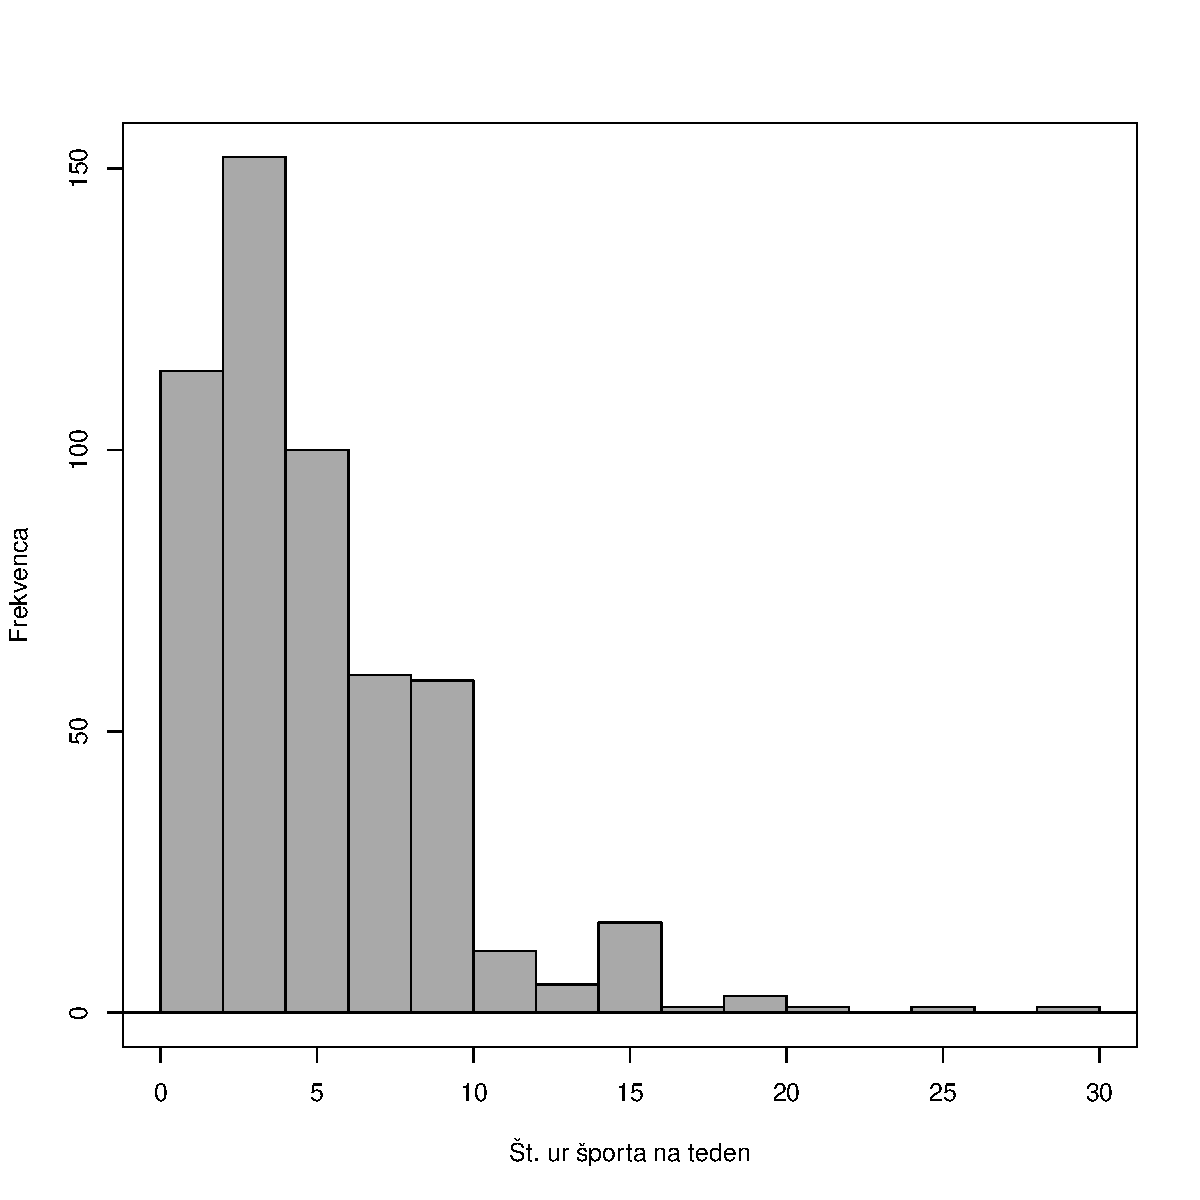
\includegraphics[width=750px]{RcmdrMarkdown_files/figure-latex/unnamed-chunk-10-1}

\begin{Shaded}
\begin{Highlighting}[]
\SpecialCharTok{\textgreater{}} \FunctionTok{with}\NormalTok{(Dataset, }\FunctionTok{Hist}\NormalTok{(Sport..hours.per.week., }\AttributeTok{scale=}\StringTok{"frequency"}\NormalTok{,}
\SpecialCharTok{+} \AttributeTok{breaks=}\StringTok{"Sturges"}\NormalTok{, }\AttributeTok{col=}\StringTok{"darkgray"}\NormalTok{, }\AttributeTok{xlab=}\StringTok{"Št. ur športa na teden"}\NormalTok{,}
\SpecialCharTok{+} \AttributeTok{ylab=}\StringTok{"Frekvenca"}\NormalTok{))}
\end{Highlighting}
\end{Shaded}

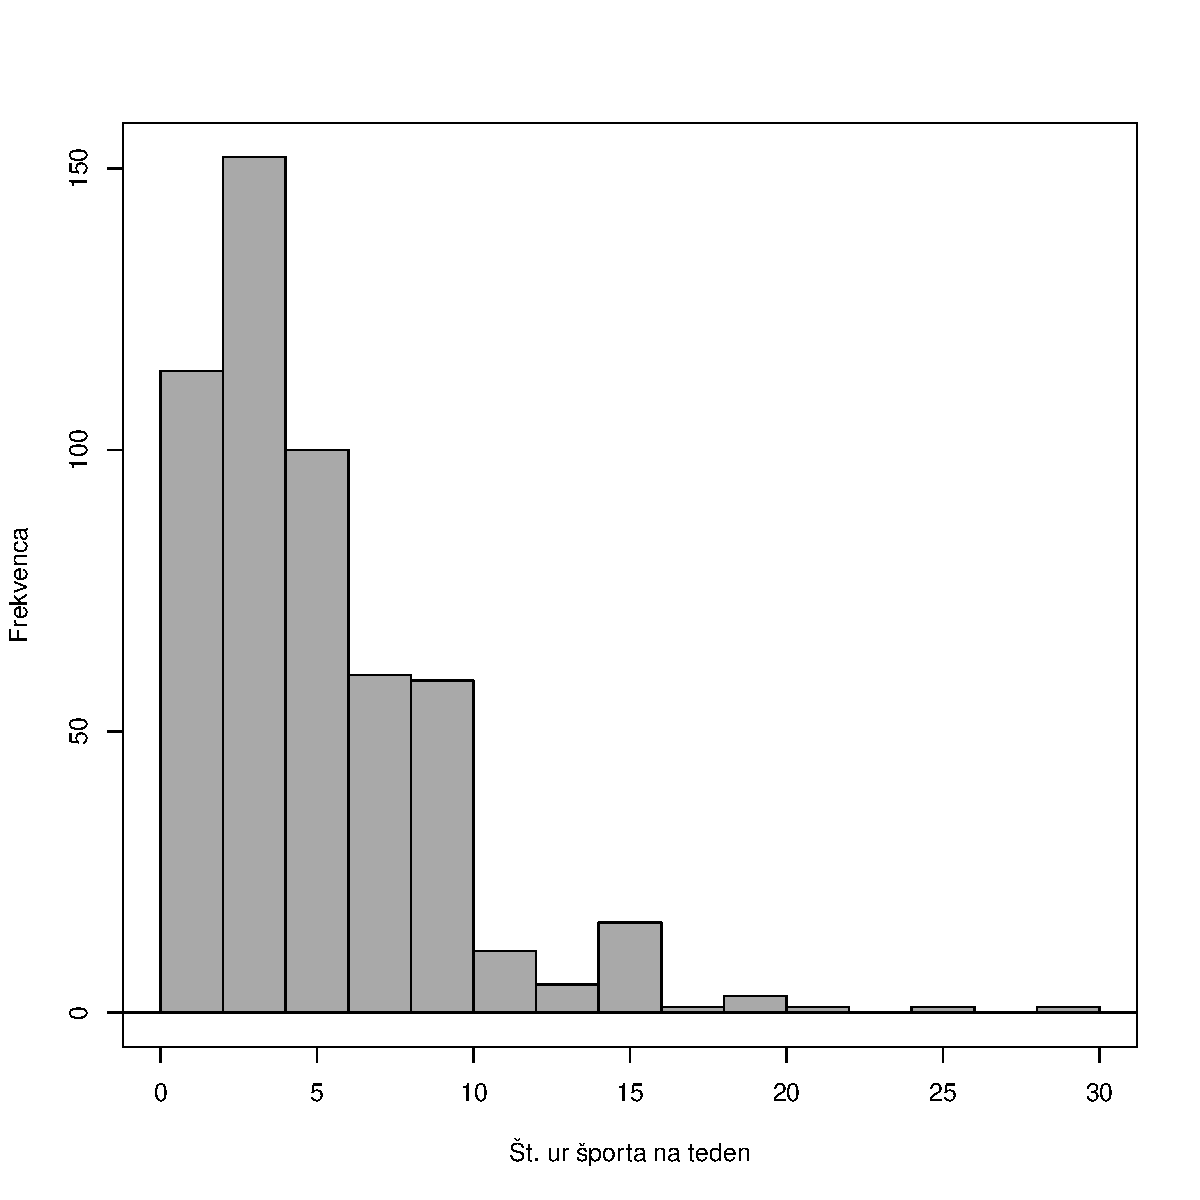
\includegraphics[width=750px]{RcmdrMarkdown_files/figure-latex/unnamed-chunk-11-1}

\subsubsection{Histogram:
Sport..hours.per.week.}\label{histogram-sport..hours.per.week.-3}

\begin{Shaded}
\begin{Highlighting}[]
\SpecialCharTok{\textgreater{}} \FunctionTok{with}\NormalTok{(Dataset, }\FunctionTok{Hist}\NormalTok{(Sport..hours.per.week., }\AttributeTok{groups=}\NormalTok{Smoking, }
\SpecialCharTok{+}   \AttributeTok{scale=}\StringTok{"frequency"}\NormalTok{, }\AttributeTok{breaks=}\StringTok{"Sturges"}\NormalTok{, }\AttributeTok{col=}\StringTok{"darkgray"}\NormalTok{, }
\SpecialCharTok{+}   \AttributeTok{xlab=}\StringTok{"Št. ur športa na teden"}\NormalTok{, }\AttributeTok{ylab=}\StringTok{"Frekvenca"}\NormalTok{))}
\end{Highlighting}
\end{Shaded}

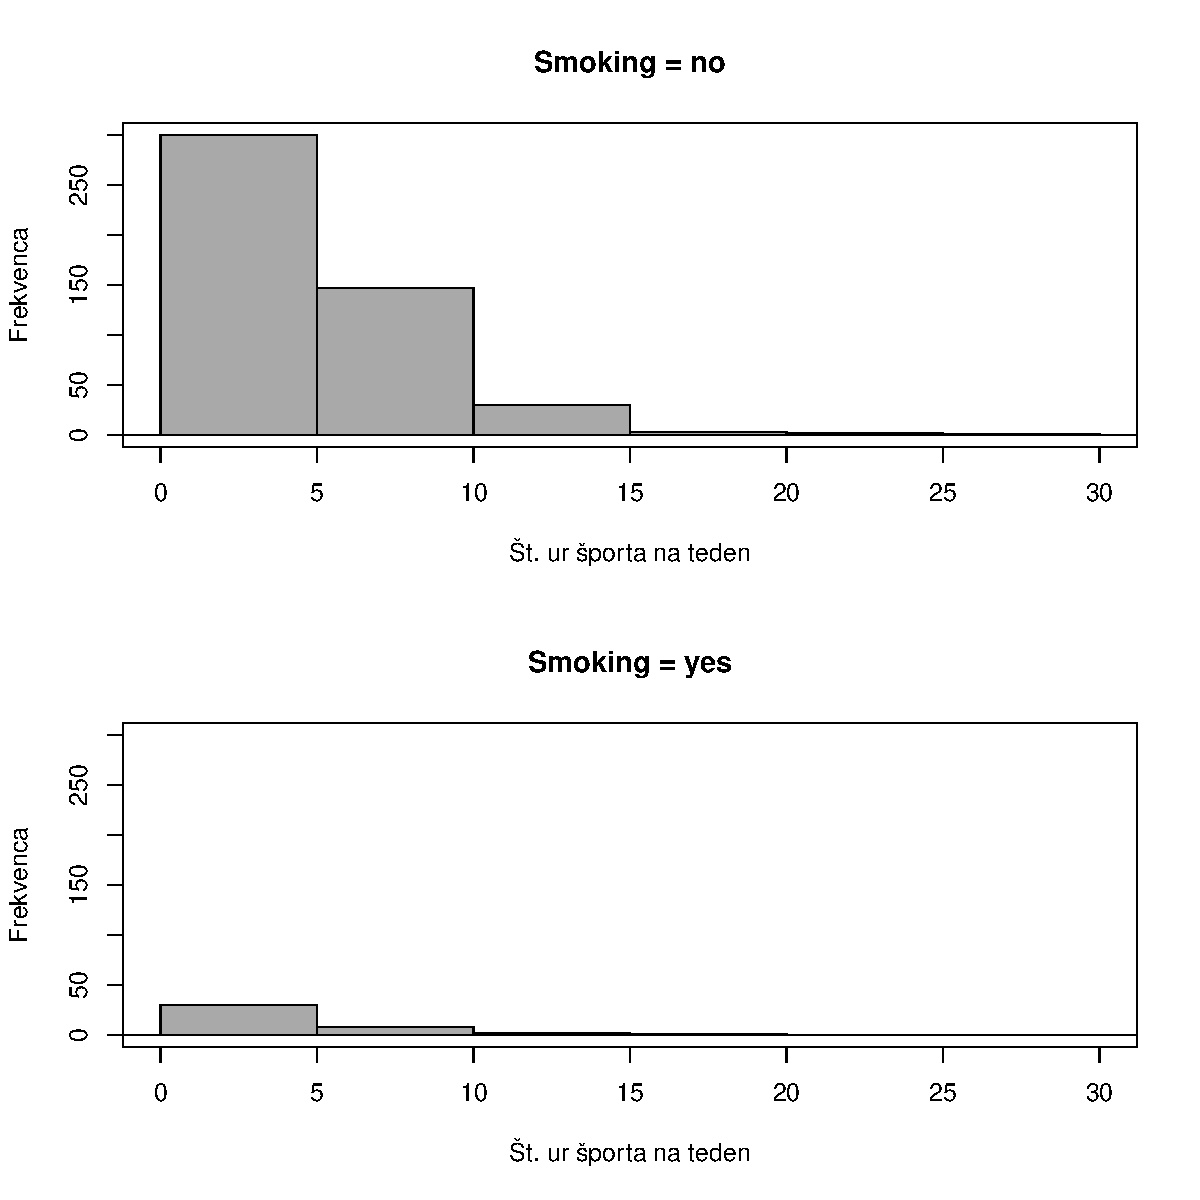
\includegraphics[width=750px]{RcmdrMarkdown_files/figure-latex/unnamed-chunk-12-1}

\subsubsection{Histogram: Weight}\label{histogram-weight}

\begin{Shaded}
\begin{Highlighting}[]
\SpecialCharTok{\textgreater{}} \FunctionTok{with}\NormalTok{(Dataset, }\FunctionTok{Hist}\NormalTok{(Weight, }\AttributeTok{groups=}\NormalTok{Videogames, }\AttributeTok{scale=}\StringTok{"frequency"}\NormalTok{, }
\SpecialCharTok{+}   \AttributeTok{breaks=}\StringTok{"Sturges"}\NormalTok{, }\AttributeTok{col=}\StringTok{"darkgray"}\NormalTok{))}
\end{Highlighting}
\end{Shaded}

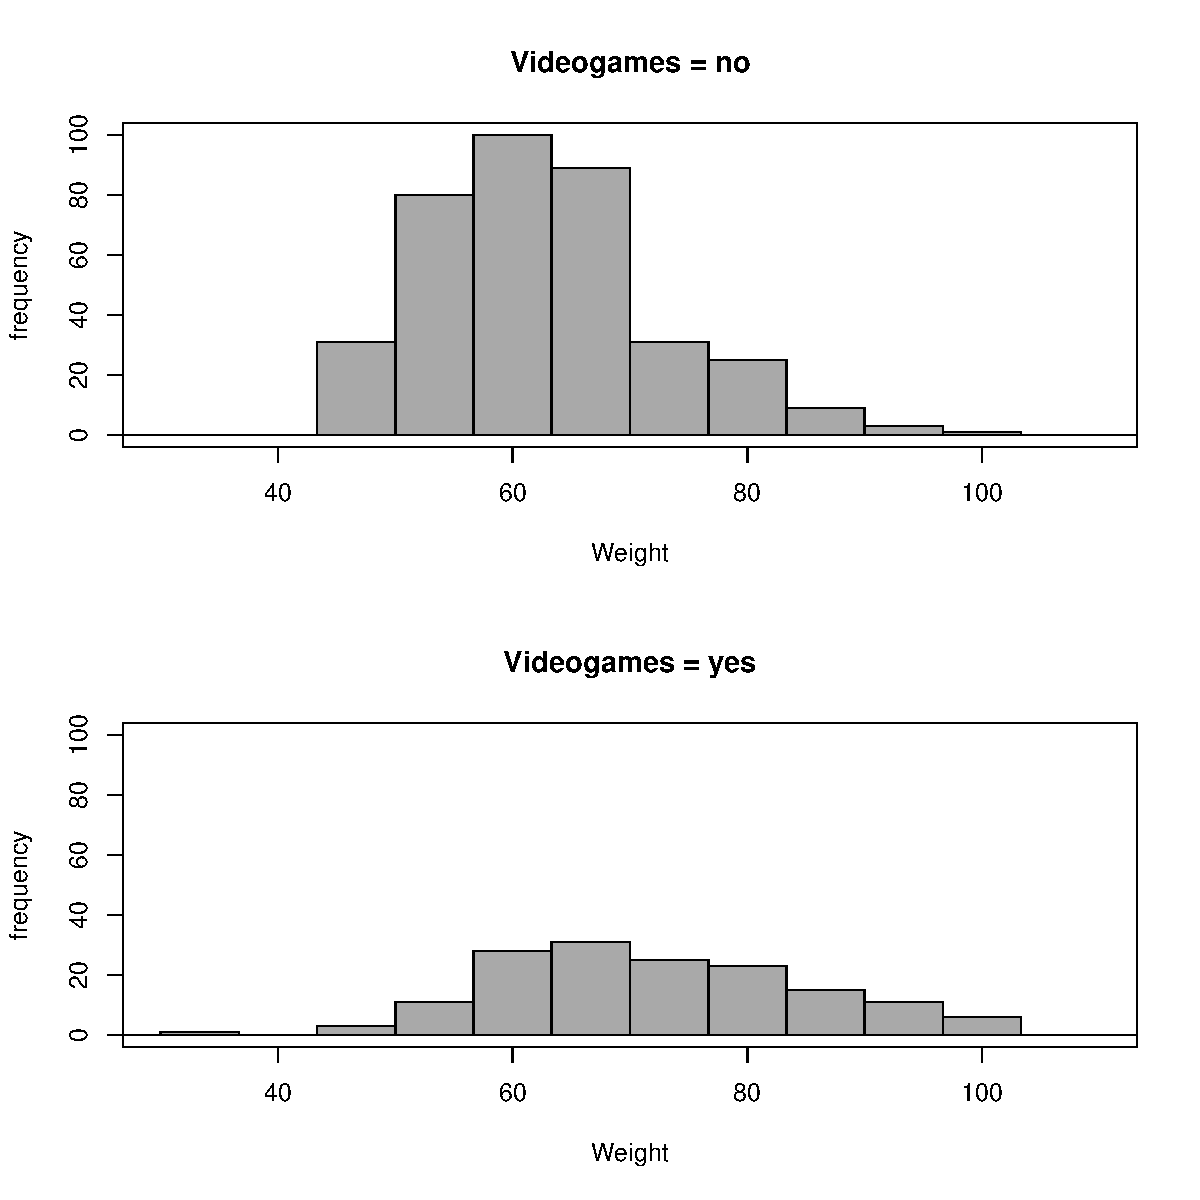
\includegraphics[width=750px]{RcmdrMarkdown_files/figure-latex/unnamed-chunk-13-1}

\subsubsection{Bar Plot: Videogames}\label{bar-plot-videogames}

\begin{Shaded}
\begin{Highlighting}[]
\SpecialCharTok{\textgreater{}} \FunctionTok{with}\NormalTok{(Dataset, }\FunctionTok{Barplot}\NormalTok{(Videogames, }\AttributeTok{by=}\NormalTok{Sex, }\AttributeTok{style=}\StringTok{"divided"}\NormalTok{, }
\SpecialCharTok{+}   \AttributeTok{legend.pos=}\StringTok{"above"}\NormalTok{, }\AttributeTok{xlab=}\StringTok{"Videogames"}\NormalTok{, }\AttributeTok{ylab=}\StringTok{"Frequency"}\NormalTok{, }\AttributeTok{label.bars=}\ConstantTok{TRUE}\NormalTok{))}
\end{Highlighting}
\end{Shaded}

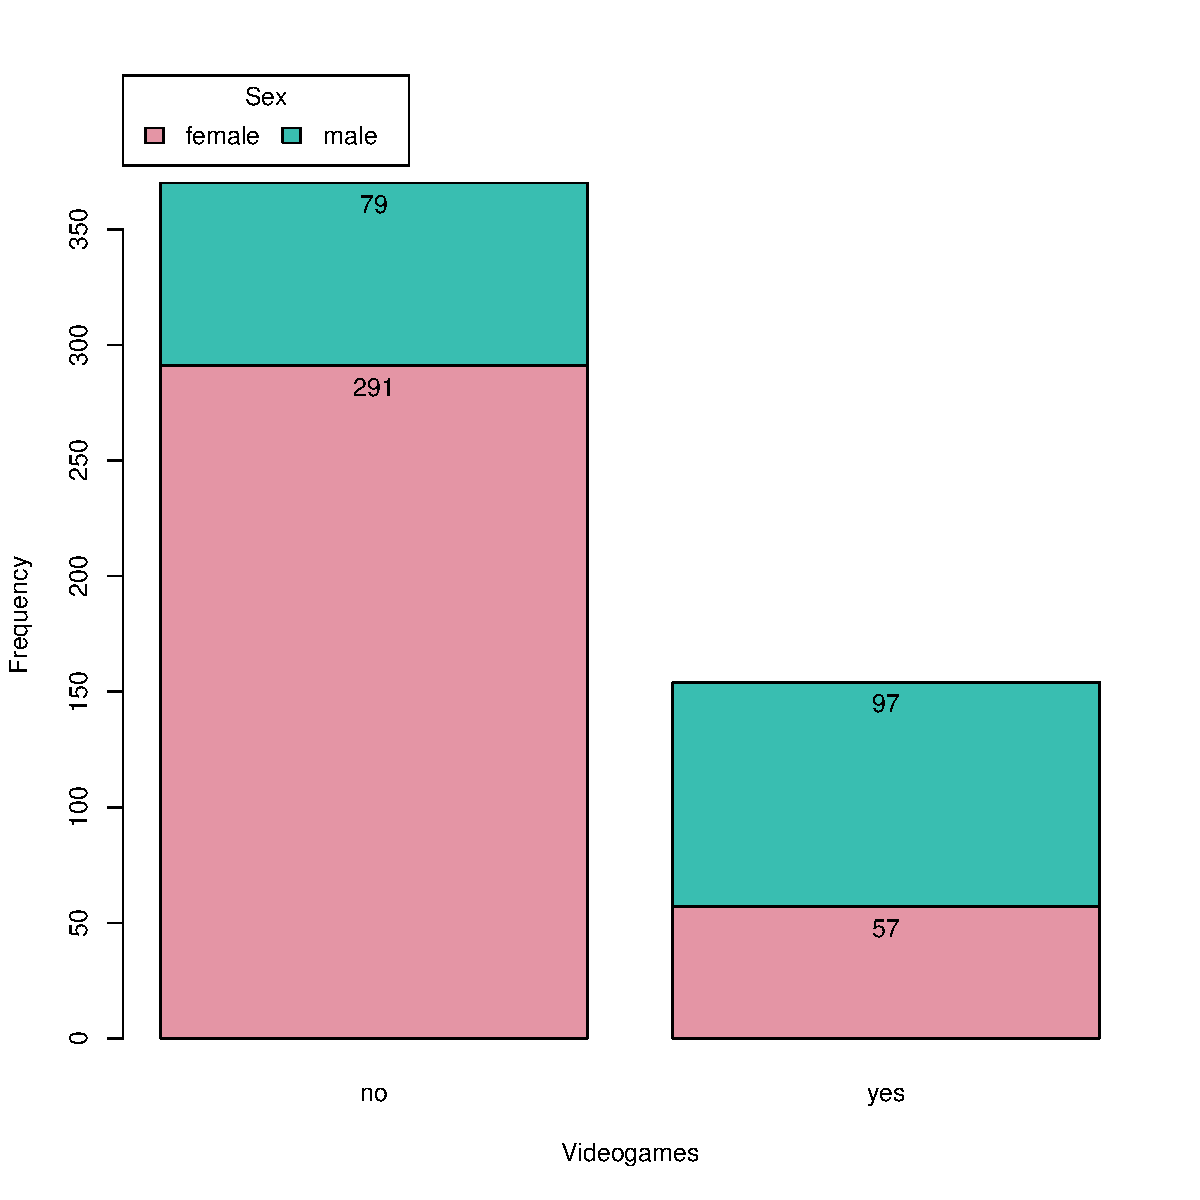
\includegraphics[width=750px]{RcmdrMarkdown_files/figure-latex/unnamed-chunk-14-1}

\subsubsection{Histogram: Weight}\label{histogram-weight-1}

\begin{Shaded}
\begin{Highlighting}[]
\SpecialCharTok{\textgreater{}} \FunctionTok{with}\NormalTok{(Dataset, }\FunctionTok{Hist}\NormalTok{(Weight, }\AttributeTok{groups=}\NormalTok{Sex, }\AttributeTok{scale=}\StringTok{"frequency"}\NormalTok{, }\AttributeTok{breaks=}\StringTok{"Sturges"}\NormalTok{, }
\SpecialCharTok{+}   \AttributeTok{col=}\StringTok{"darkgray"}\NormalTok{))}
\end{Highlighting}
\end{Shaded}

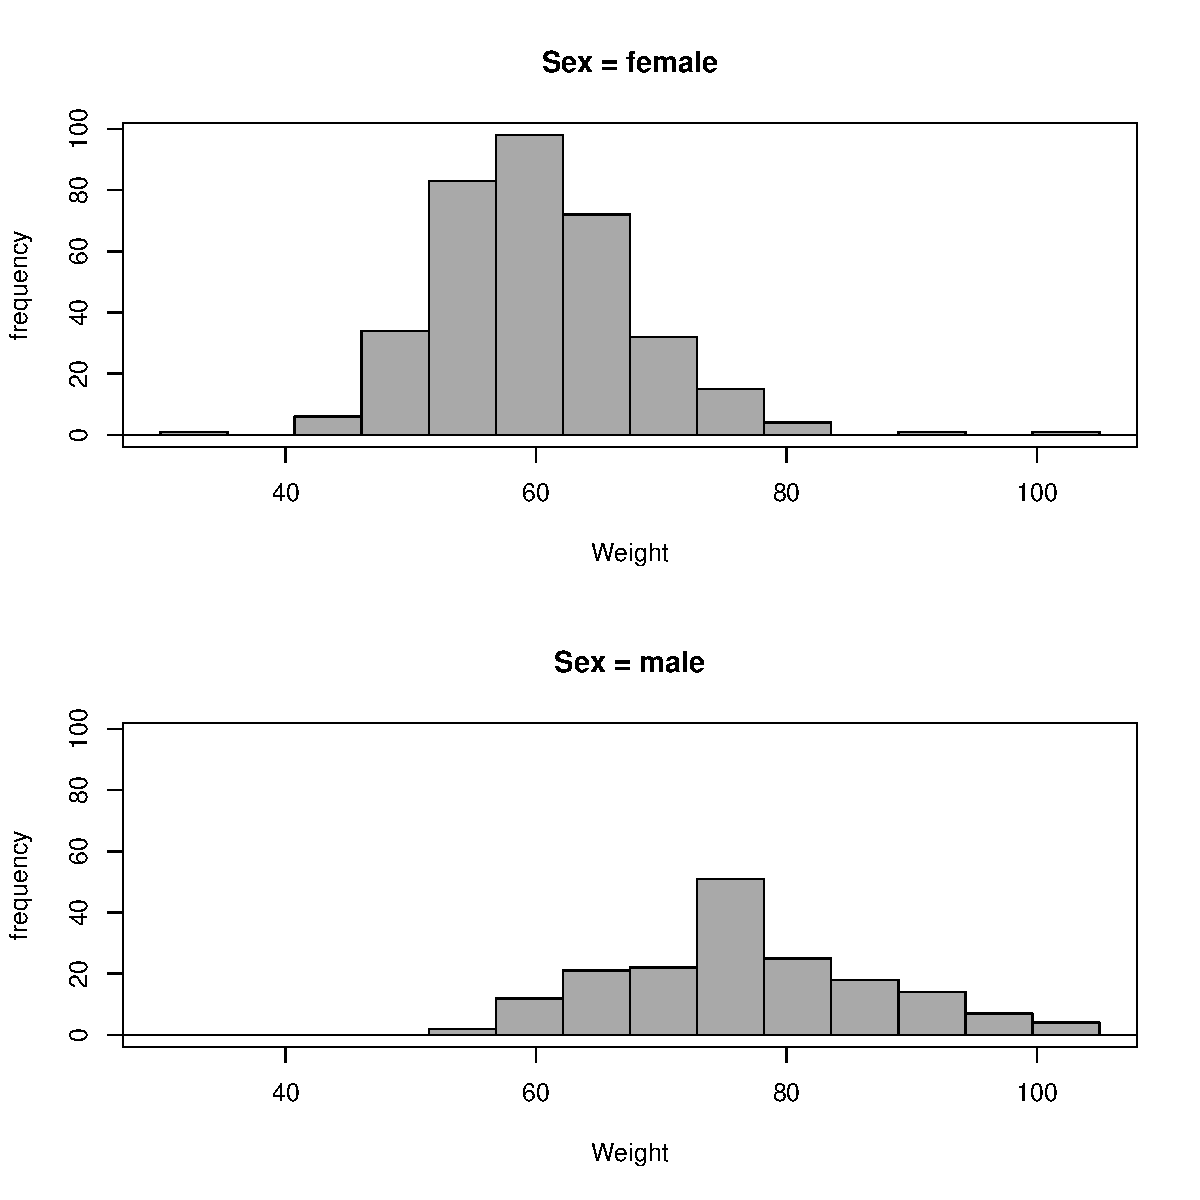
\includegraphics[width=750px]{RcmdrMarkdown_files/figure-latex/unnamed-chunk-15-1}

\subsubsection{Histogram:
Friends.on.Facebook}\label{histogram-friends.on.facebook}

\begin{Shaded}
\begin{Highlighting}[]
\SpecialCharTok{\textgreater{}} \FunctionTok{with}\NormalTok{(Dataset, }\FunctionTok{Hist}\NormalTok{(Friends.on.Facebook, }\AttributeTok{groups=}\NormalTok{Videogames, }
\SpecialCharTok{+}   \AttributeTok{scale=}\StringTok{"frequency"}\NormalTok{, }\AttributeTok{breaks=}\StringTok{"Sturges"}\NormalTok{, }\AttributeTok{col=}\StringTok{"darkgray"}\NormalTok{))}
\end{Highlighting}
\end{Shaded}

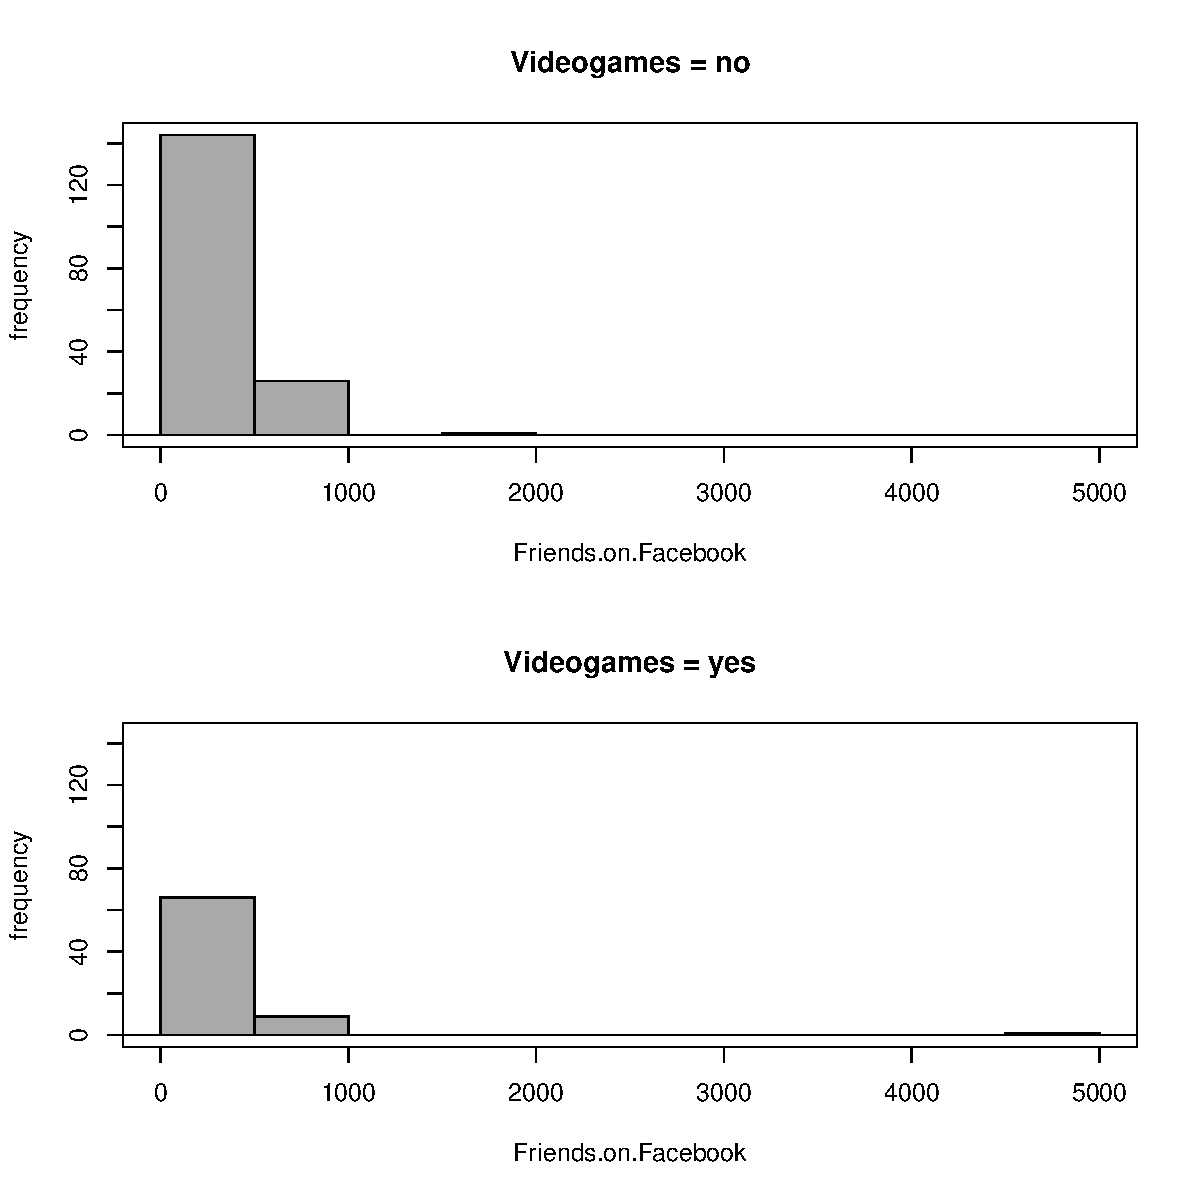
\includegraphics[width=750px]{RcmdrMarkdown_files/figure-latex/unnamed-chunk-16-1}

\subsubsection{Bar Plot: Eye.Color}\label{bar-plot-eye.color}

\begin{Shaded}
\begin{Highlighting}[]
\SpecialCharTok{\textgreater{}} \FunctionTok{with}\NormalTok{(Dataset, }\FunctionTok{Barplot}\NormalTok{(Eye.Color, }\AttributeTok{by=}\NormalTok{Sex, }\AttributeTok{style=}\StringTok{"divided"}\NormalTok{, }
\SpecialCharTok{+}   \AttributeTok{legend.pos=}\StringTok{"above"}\NormalTok{, }\AttributeTok{xlab=}\StringTok{"Eye.Color"}\NormalTok{, }\AttributeTok{ylab=}\StringTok{"Frequency"}\NormalTok{, }\AttributeTok{label.bars=}\ConstantTok{TRUE}\NormalTok{))}
\end{Highlighting}
\end{Shaded}

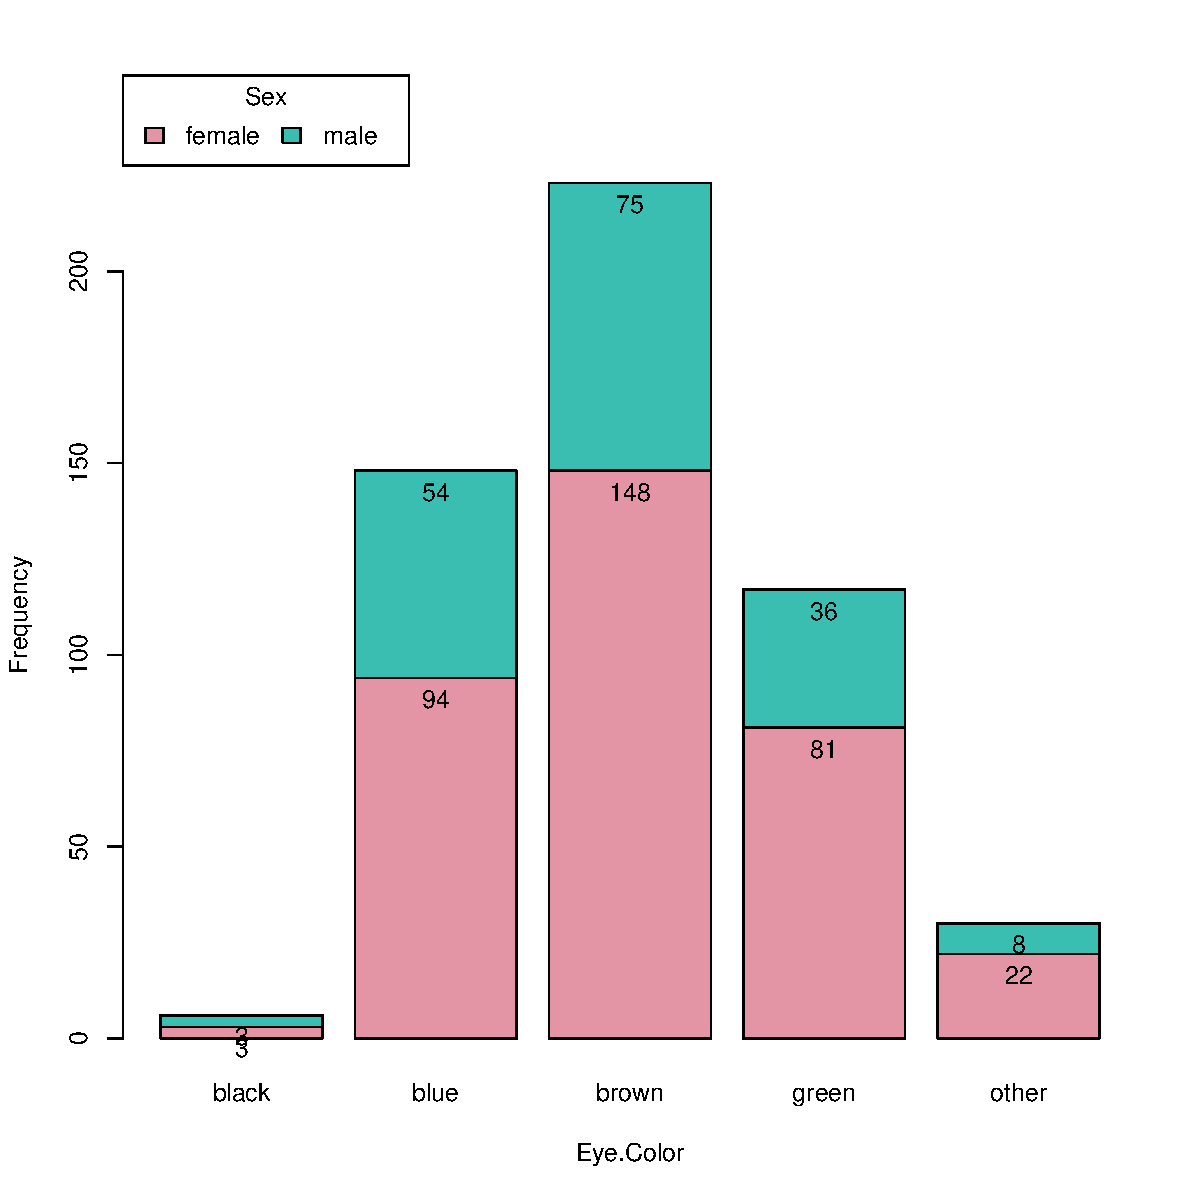
\includegraphics[width=750px]{RcmdrMarkdown_files/figure-latex/unnamed-chunk-17-1}

\subsubsection{Bar Plot: Eye.Color}\label{bar-plot-eye.color-1}

\begin{Shaded}
\begin{Highlighting}[]
\SpecialCharTok{\textgreater{}} \FunctionTok{with}\NormalTok{(Dataset, }\FunctionTok{Barplot}\NormalTok{(Eye.Color, }\AttributeTok{xlab=}\StringTok{"Eye.Color"}\NormalTok{, }\AttributeTok{ylab=}\StringTok{"Frequency"}\NormalTok{, }
\SpecialCharTok{+}   \AttributeTok{label.bars=}\ConstantTok{TRUE}\NormalTok{))}
\end{Highlighting}
\end{Shaded}

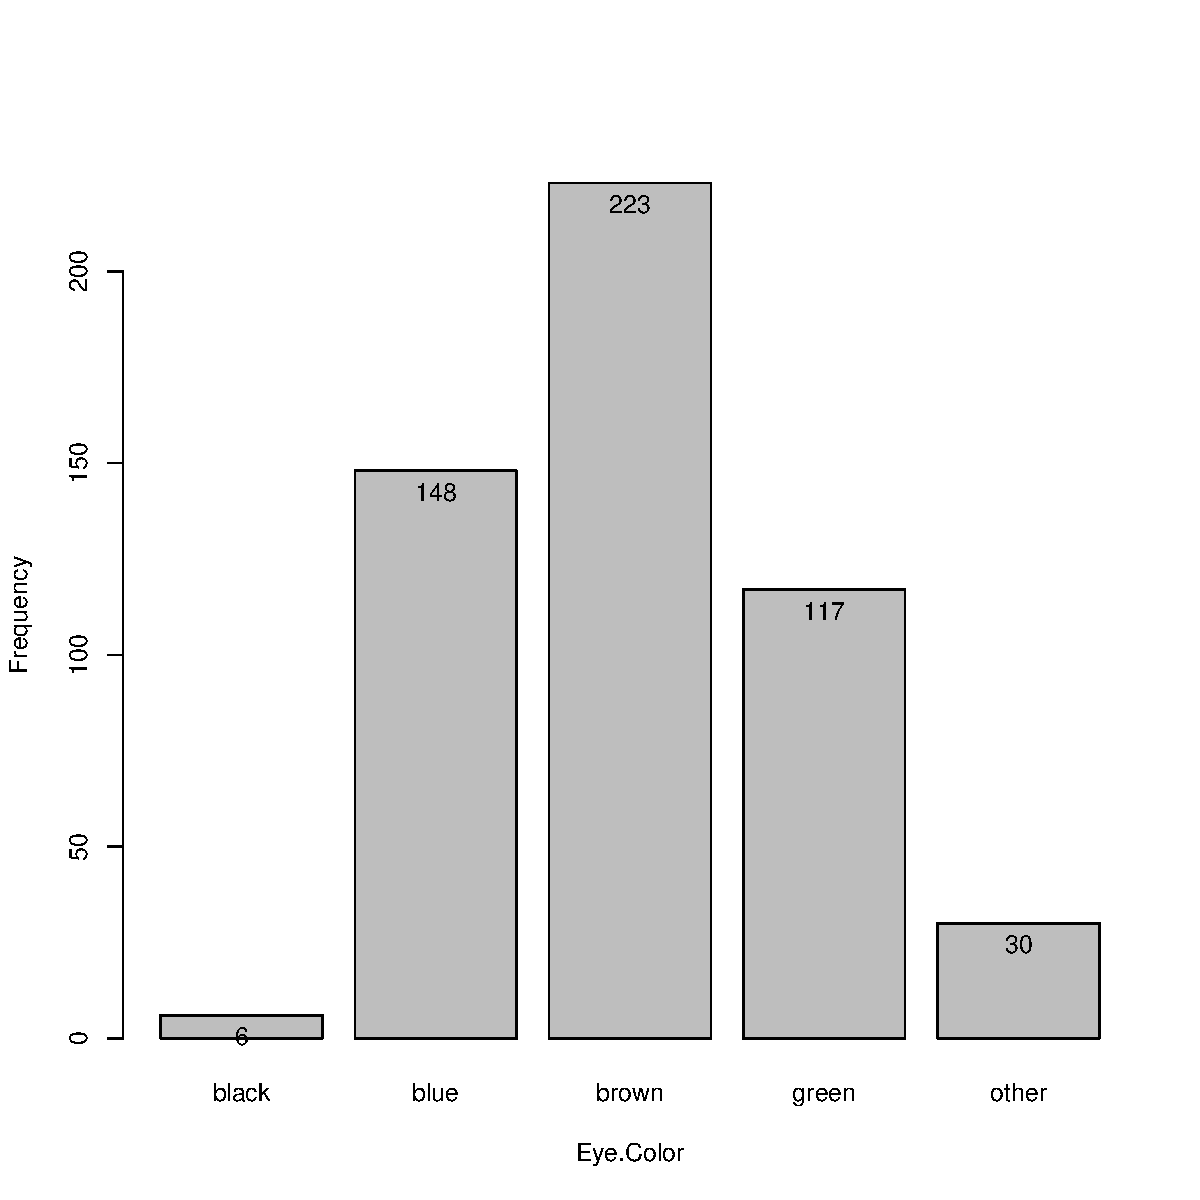
\includegraphics[width=750px]{RcmdrMarkdown_files/figure-latex/unnamed-chunk-18-1}

\begin{Shaded}
\begin{Highlighting}[]
\SpecialCharTok{\textgreater{}} \FunctionTok{library}\NormalTok{(colorspace, }\AttributeTok{pos=}\DecValTok{19}\NormalTok{)}
\end{Highlighting}
\end{Shaded}

\subsubsection{Pie Chart: Eye.Color}\label{pie-chart-eye.color}

\begin{Shaded}
\begin{Highlighting}[]
\SpecialCharTok{\textgreater{}} \FunctionTok{with}\NormalTok{(Dataset, }\FunctionTok{piechart}\NormalTok{(Eye.Color, }\AttributeTok{xlab=}\StringTok{""}\NormalTok{, }\AttributeTok{ylab=}\StringTok{""}\NormalTok{, }\AttributeTok{main=}\StringTok{"Eye.Color"}\NormalTok{, }
\SpecialCharTok{+}   \AttributeTok{col=}\FunctionTok{rainbow\_hcl}\NormalTok{(}\DecValTok{5}\NormalTok{), }\AttributeTok{scale=}\StringTok{"percent"}\NormalTok{))}
\end{Highlighting}
\end{Shaded}

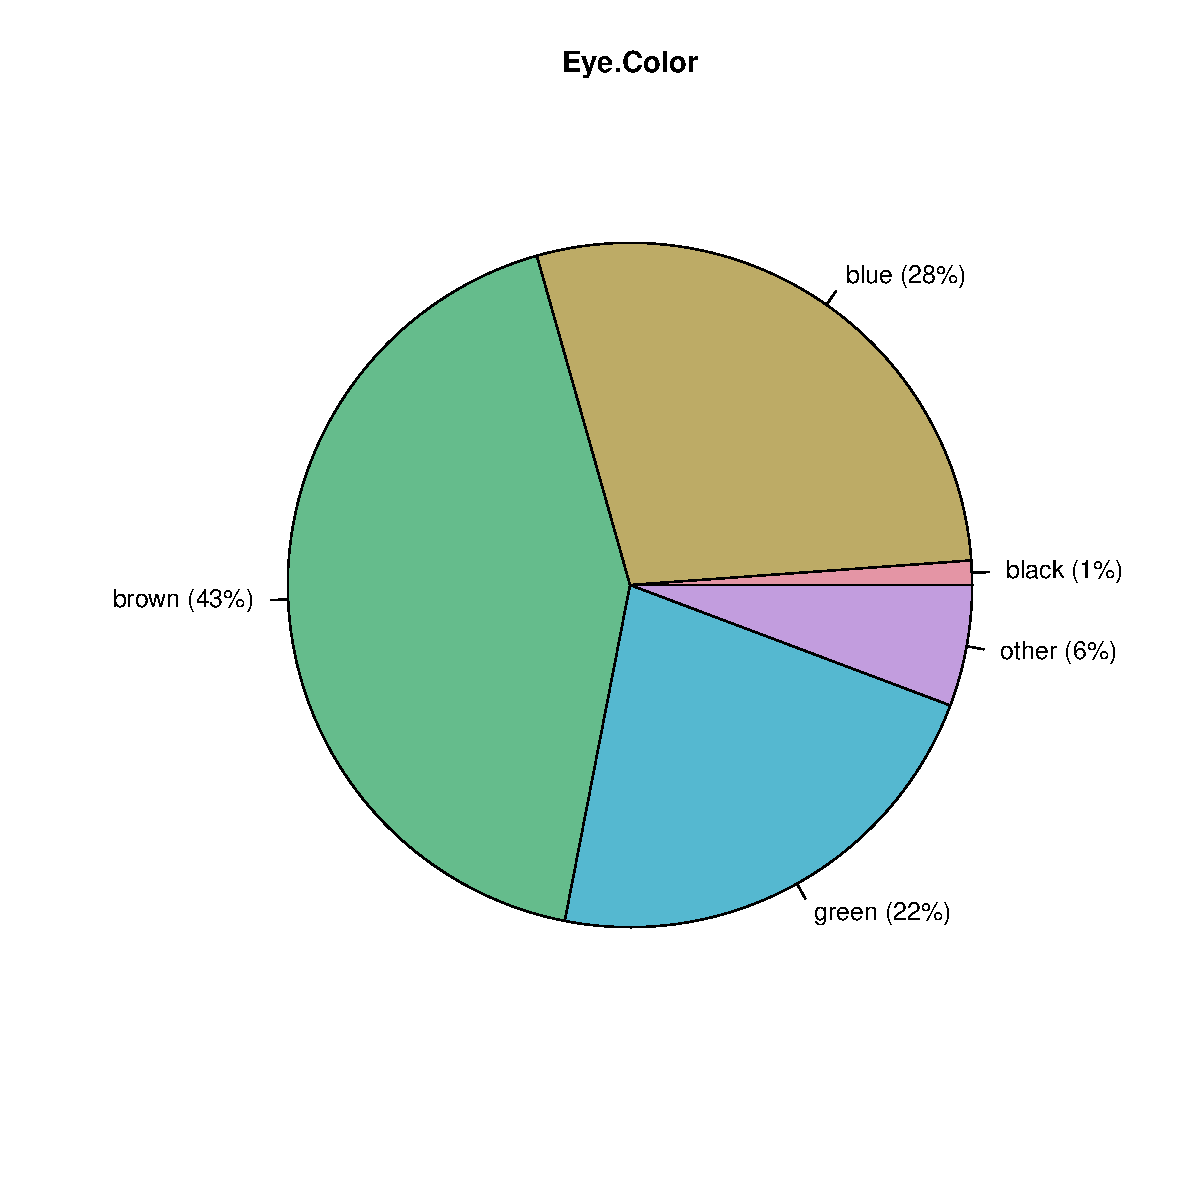
\includegraphics[width=750px]{RcmdrMarkdown_files/figure-latex/unnamed-chunk-20-1}

\subsubsection{Pie Chart: Eye.Color}\label{pie-chart-eye.color-1}

\begin{Shaded}
\begin{Highlighting}[]
\SpecialCharTok{\textgreater{}} \FunctionTok{with}\NormalTok{(Dataset, }\FunctionTok{piechart}\NormalTok{(Eye.Color, }\AttributeTok{xlab=}\StringTok{""}\NormalTok{, }\AttributeTok{ylab=}\StringTok{""}\NormalTok{, }\AttributeTok{main=}\StringTok{"Eye.Color"}\NormalTok{, }
\SpecialCharTok{+}   \AttributeTok{col=}\FunctionTok{palette}\NormalTok{()[}\DecValTok{2}\SpecialCharTok{:}\DecValTok{6}\NormalTok{], }\AttributeTok{scale=}\StringTok{"percent"}\NormalTok{))}
\end{Highlighting}
\end{Shaded}

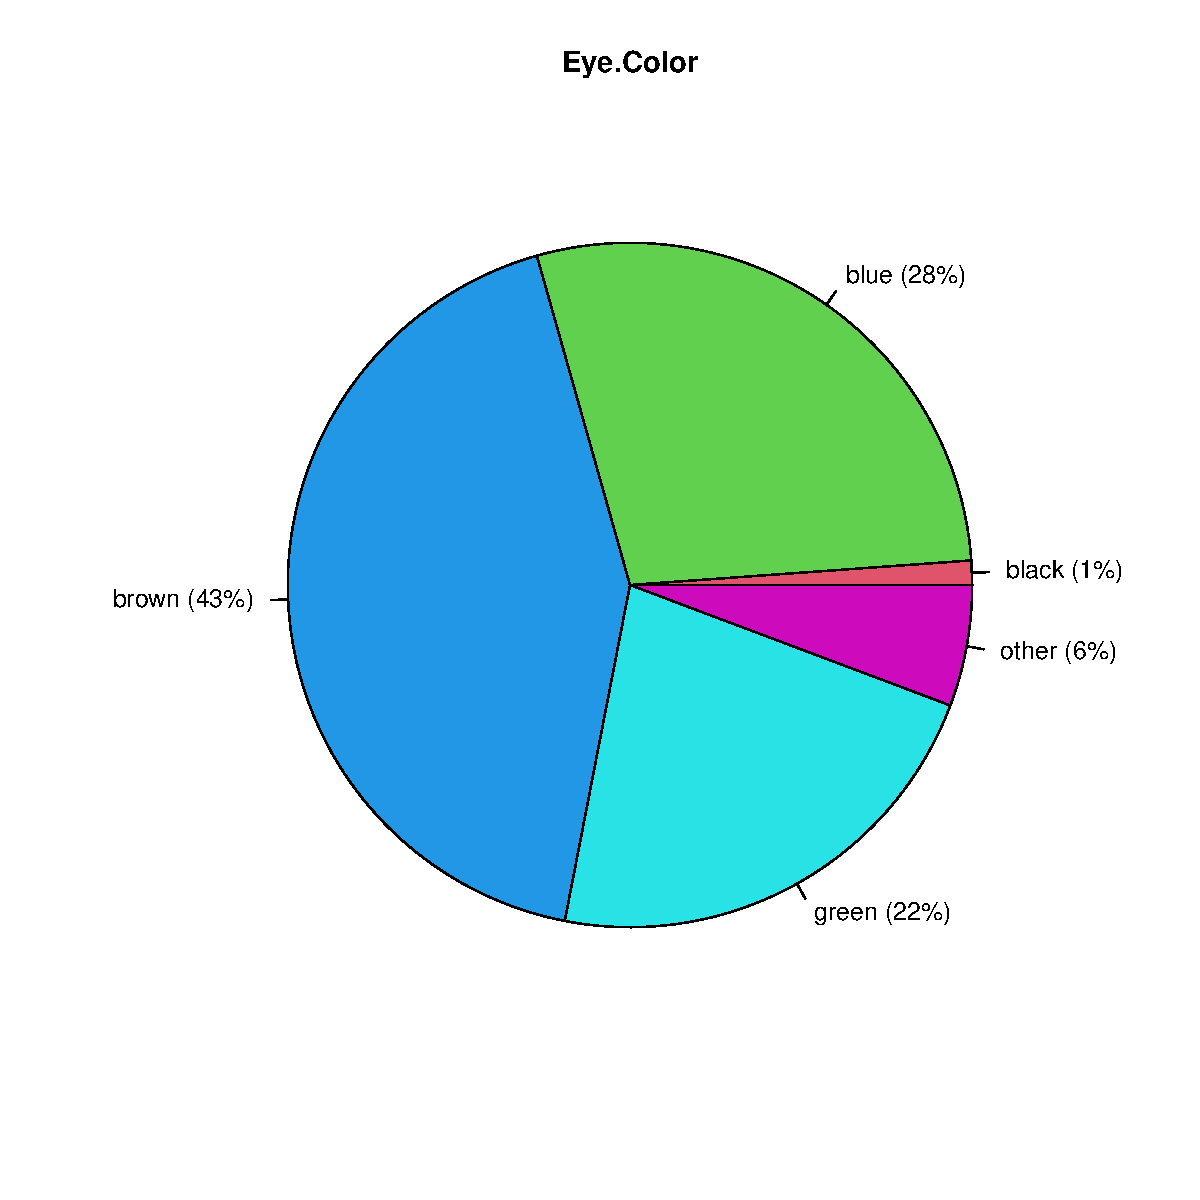
\includegraphics[width=750px]{RcmdrMarkdown_files/figure-latex/unnamed-chunk-21-1}

\subsubsection{Pie Chart: Eye.Color}\label{pie-chart-eye.color-2}

\begin{Shaded}
\begin{Highlighting}[]
\SpecialCharTok{\textgreater{}} \FunctionTok{with}\NormalTok{(Dataset, }\FunctionTok{piechart}\NormalTok{(Eye.Color, }\AttributeTok{xlab=}\StringTok{""}\NormalTok{, }\AttributeTok{ylab=}\StringTok{""}\NormalTok{, }\AttributeTok{main=}\StringTok{"Eye.Color"}\NormalTok{, }
\SpecialCharTok{+}   \AttributeTok{col=}\FunctionTok{palette}\NormalTok{()[}\DecValTok{2}\SpecialCharTok{:}\DecValTok{6}\NormalTok{], }\AttributeTok{scale=}\StringTok{"percent"}\NormalTok{))}
\end{Highlighting}
\end{Shaded}

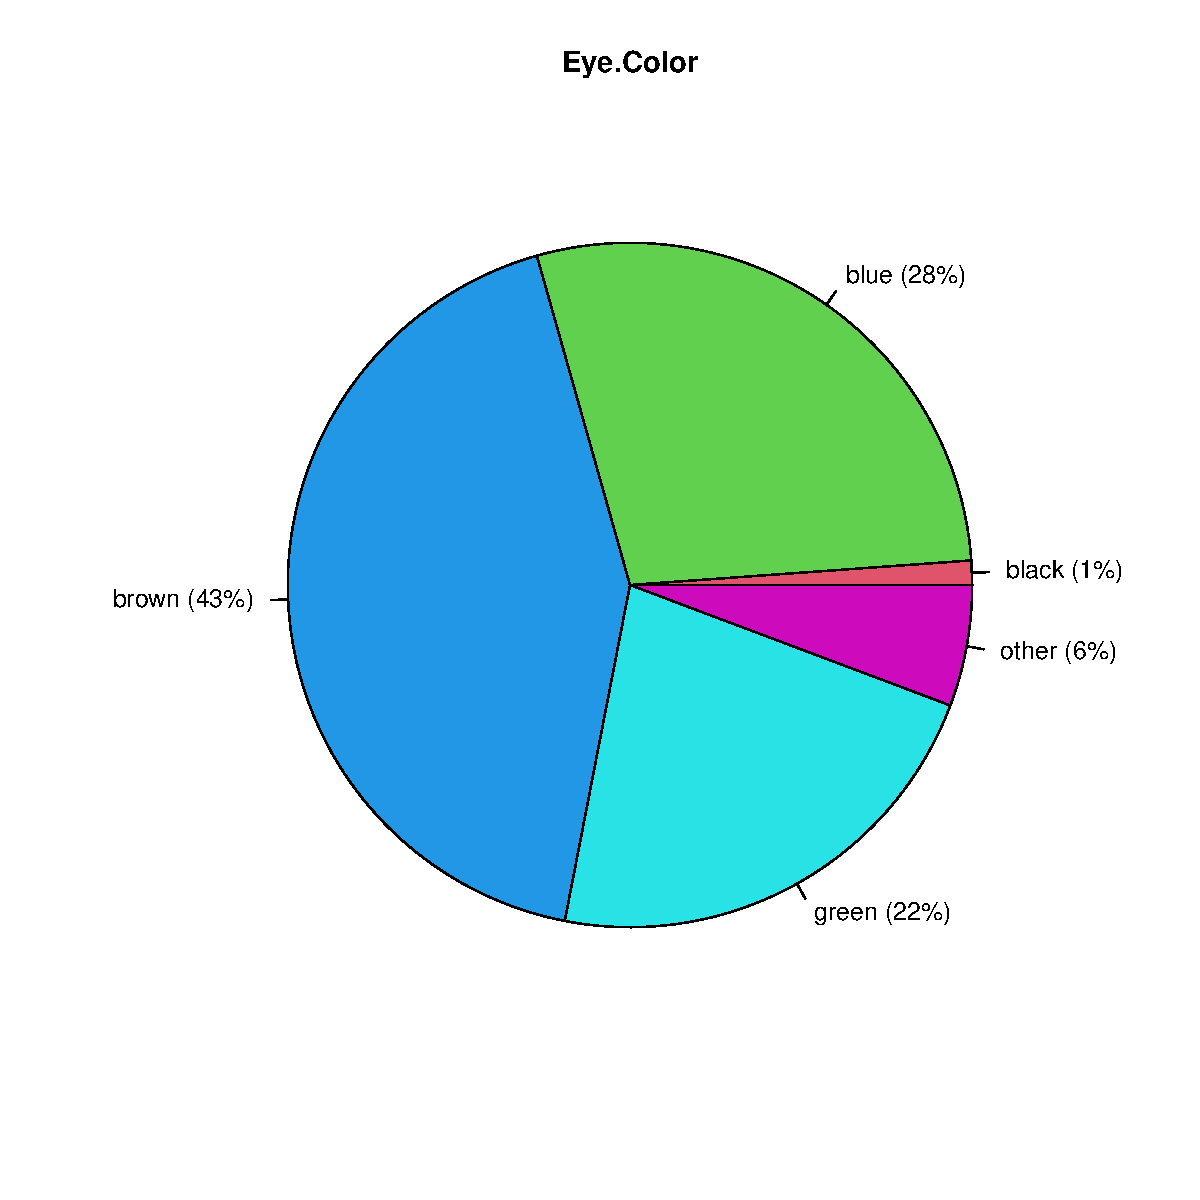
\includegraphics[width=750px]{RcmdrMarkdown_files/figure-latex/unnamed-chunk-22-1}

\subsubsection{Bar Plot: Sex}\label{bar-plot-sex}

\begin{Shaded}
\begin{Highlighting}[]
\SpecialCharTok{\textgreater{}} \FunctionTok{with}\NormalTok{(Dataset, }\FunctionTok{Barplot}\NormalTok{(Sex, }\AttributeTok{by=}\NormalTok{Faculty, }\AttributeTok{style=}\StringTok{"divided"}\NormalTok{, }\AttributeTok{legend.pos=}\StringTok{"above"}\NormalTok{, }
\SpecialCharTok{+}   \AttributeTok{xlab=}\StringTok{"Sex"}\NormalTok{, }\AttributeTok{ylab=}\StringTok{"Frequency"}\NormalTok{, }\AttributeTok{label.bars=}\ConstantTok{TRUE}\NormalTok{))}
\end{Highlighting}
\end{Shaded}

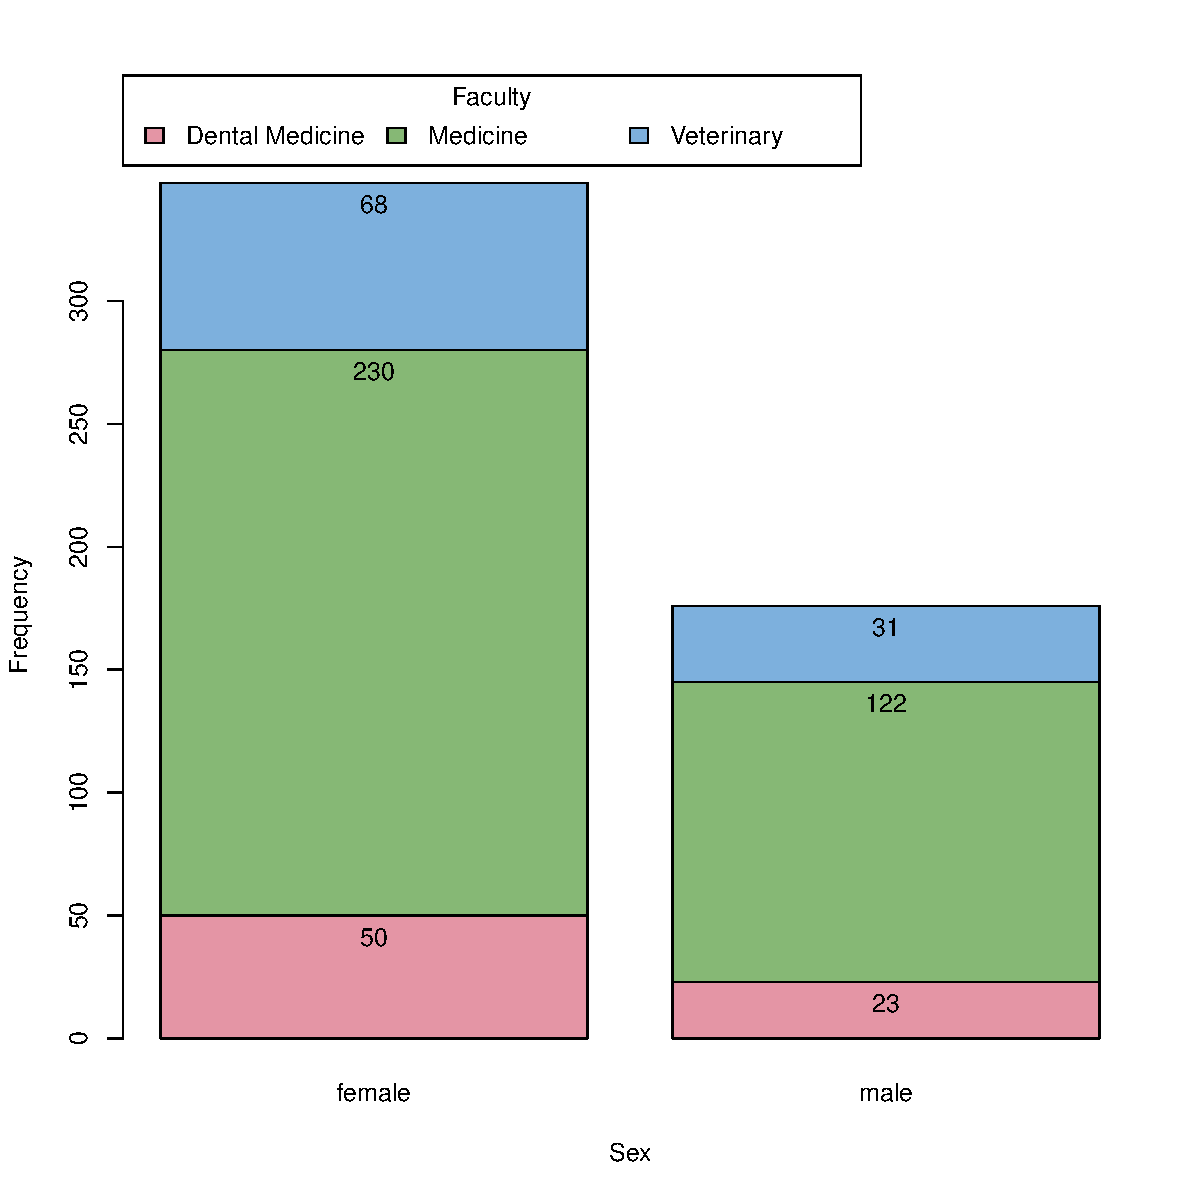
\includegraphics[width=750px]{RcmdrMarkdown_files/figure-latex/unnamed-chunk-23-1}

\subsubsection{Scatterplot:
Height\textasciitilde Weight}\label{scatterplot-heightweight}

\begin{Shaded}
\begin{Highlighting}[]
\SpecialCharTok{\textgreater{}} \FunctionTok{scatterplot}\NormalTok{(Height}\SpecialCharTok{\textasciitilde{}}\NormalTok{Weight, }\AttributeTok{regLine=}\ConstantTok{FALSE}\NormalTok{, }\AttributeTok{smooth=}\ConstantTok{FALSE}\NormalTok{, }\AttributeTok{boxplots=}\ConstantTok{FALSE}\NormalTok{, }
\SpecialCharTok{+}   \AttributeTok{data=}\NormalTok{Dataset)}
\end{Highlighting}
\end{Shaded}

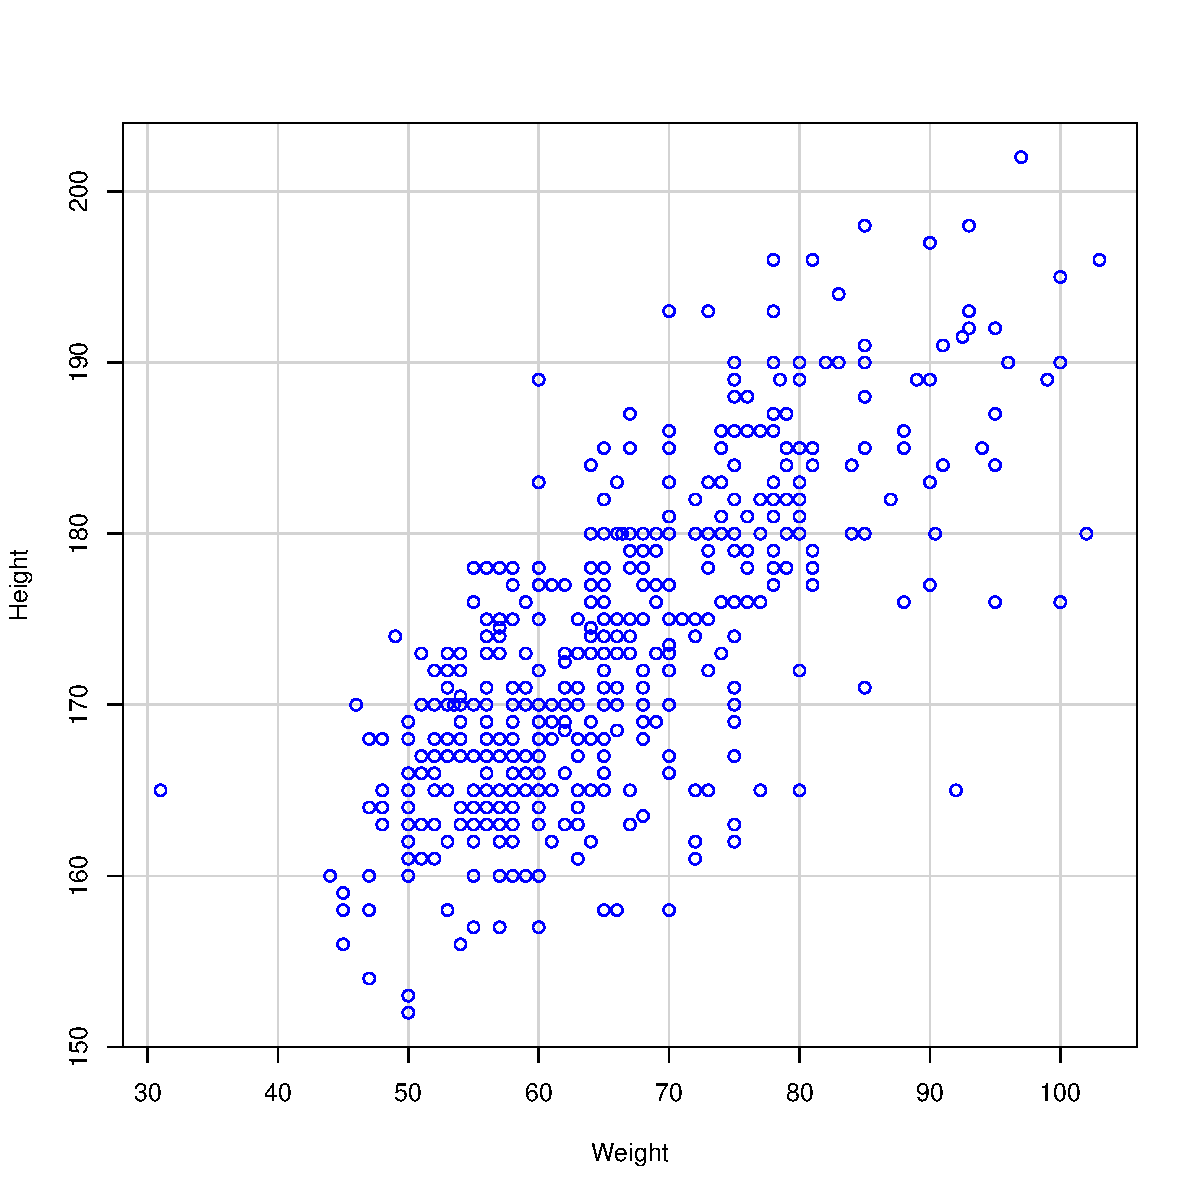
\includegraphics[width=750px]{RcmdrMarkdown_files/figure-latex/unnamed-chunk-24-1}

\subsubsection{Scatterplot:
Weight\textasciitilde Height}\label{scatterplot-weightheight}

\begin{Shaded}
\begin{Highlighting}[]
\SpecialCharTok{\textgreater{}} \FunctionTok{scatterplot}\NormalTok{(Weight}\SpecialCharTok{\textasciitilde{}}\NormalTok{Height, }\AttributeTok{regLine=}\ConstantTok{FALSE}\NormalTok{, }\AttributeTok{smooth=}\ConstantTok{FALSE}\NormalTok{, }\AttributeTok{boxplots=}\ConstantTok{FALSE}\NormalTok{, }
\SpecialCharTok{+}   \AttributeTok{data=}\NormalTok{Dataset)}
\end{Highlighting}
\end{Shaded}

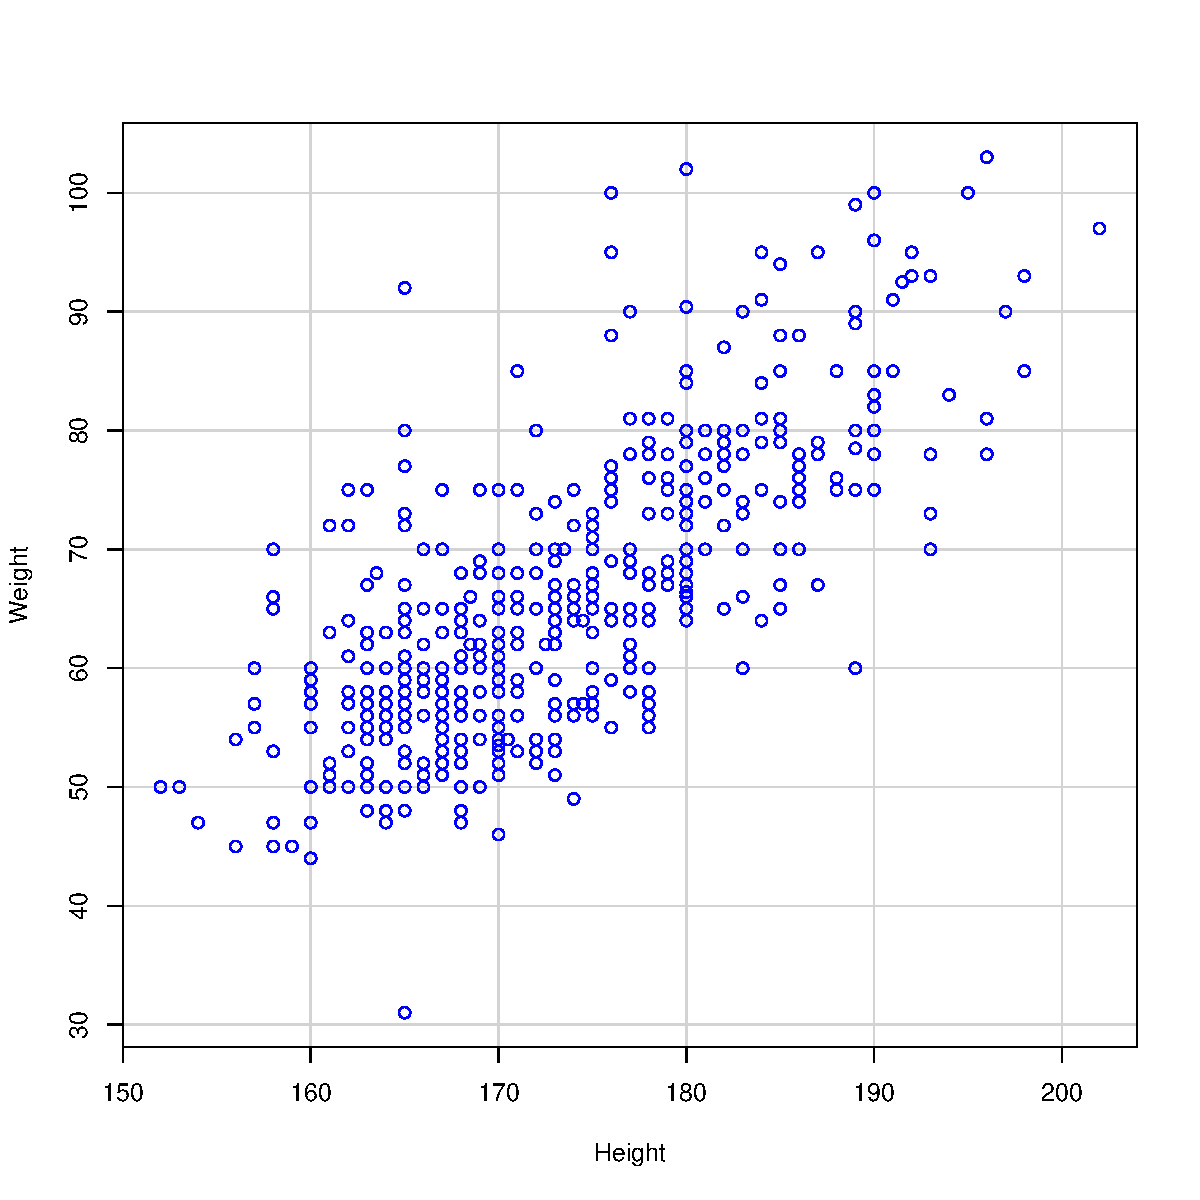
\includegraphics[width=750px]{RcmdrMarkdown_files/figure-latex/unnamed-chunk-25-1}

\subsubsection{Numerical Summaries:
Dataset}\label{numerical-summaries-dataset}

\begin{Shaded}
\begin{Highlighting}[]
\SpecialCharTok{\textgreater{}} \FunctionTok{numSummary}\NormalTok{(Dataset[,}\StringTok{"Friends.on.Facebook"}\NormalTok{, }\AttributeTok{drop=}\ConstantTok{FALSE}\NormalTok{], }\AttributeTok{statistics=}\FunctionTok{c}\NormalTok{(}\StringTok{"mean"}\NormalTok{,}
\SpecialCharTok{+}    \StringTok{"sd"}\NormalTok{, }\StringTok{"IQR"}\NormalTok{, }\StringTok{"quantiles"}\NormalTok{), }\AttributeTok{quantiles=}\FunctionTok{c}\NormalTok{(}\DecValTok{0}\NormalTok{,.}\DecValTok{25}\NormalTok{,.}\DecValTok{5}\NormalTok{,.}\DecValTok{75}\NormalTok{,}\DecValTok{1}\NormalTok{))}
\end{Highlighting}
\end{Shaded}

\begin{verbatim}
     mean       sd IQR 0% 25% 50% 75% 100%   n  NA
 325.9514 370.7482 279  0 152 300 431 5000 247 277
\end{verbatim}

\subsubsection{Boxplot: \textasciitilde{}
Friends.on.Facebook}\label{boxplot-friends.on.facebook}

\begin{Shaded}
\begin{Highlighting}[]
\SpecialCharTok{\textgreater{}} \FunctionTok{Boxplot}\NormalTok{( }\SpecialCharTok{\textasciitilde{}}\NormalTok{ Friends.on.Facebook, }\AttributeTok{data=}\NormalTok{Dataset, }\AttributeTok{id=}\FunctionTok{list}\NormalTok{(}\AttributeTok{method=}\StringTok{"y"}\NormalTok{))}
\end{Highlighting}
\end{Shaded}

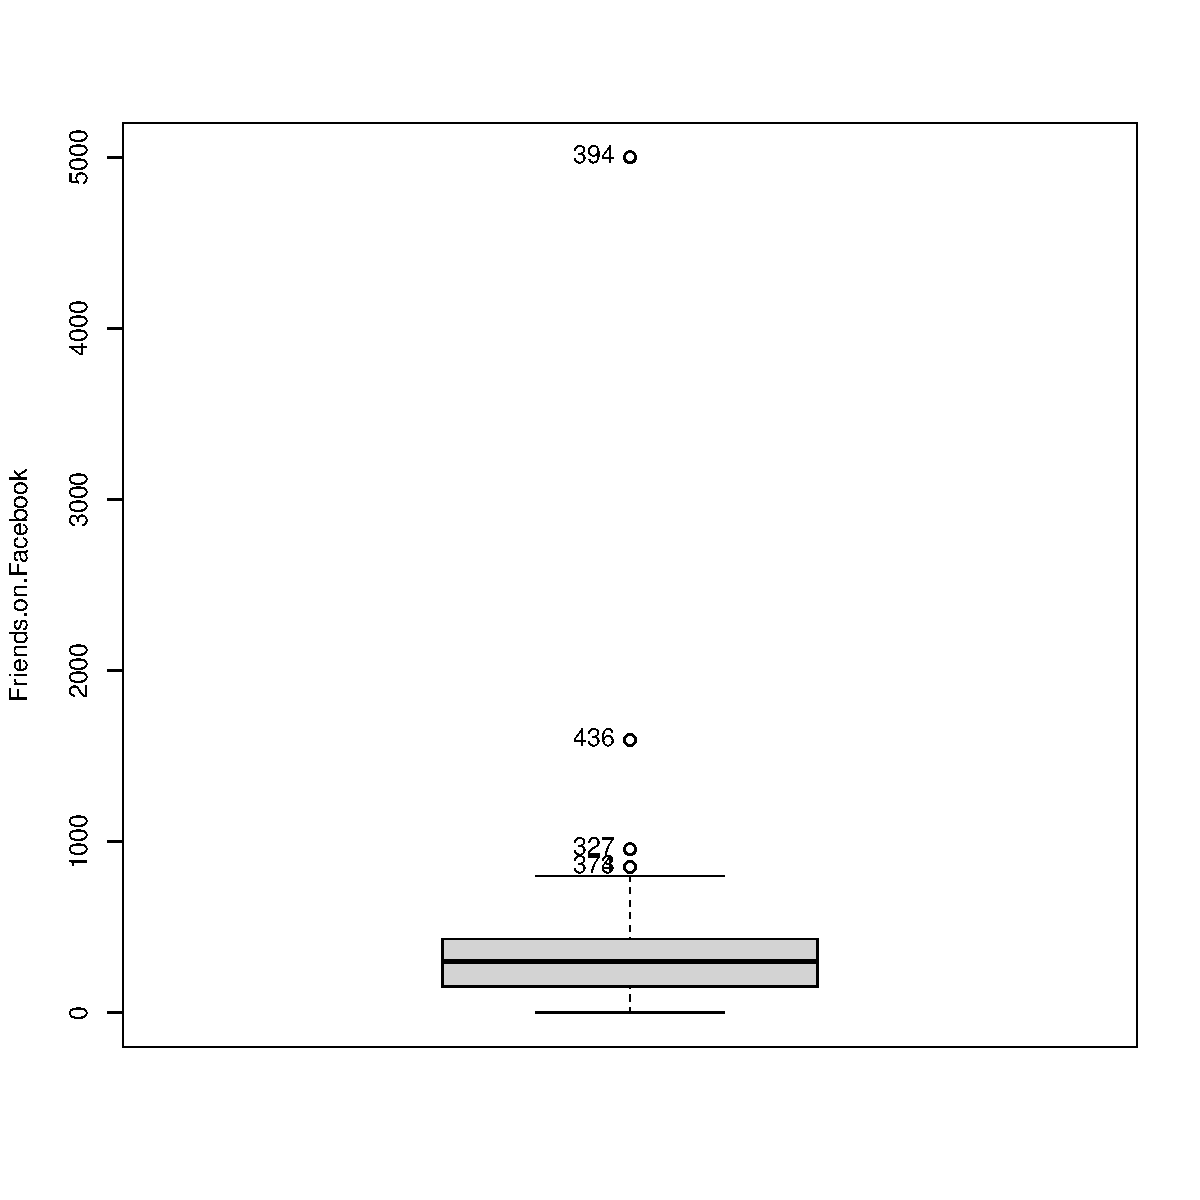
\includegraphics[width=750px]{RcmdrMarkdown_files/figure-latex/unnamed-chunk-27-1}

\begin{verbatim}
[1] "327" "373" "374" "394" "436"
\end{verbatim}

\end{document}
